\documentclass[english,12pt]{article}

% LAYOUT
\usepackage{mylayout}
\setmainlanguage{english}
\usepackage{csquotes}
\def\herospath{/usr/share/texmf/fonts/opentype/public/tex-gyre/}
\def\bibpath{bibliography.bib}
\InputIfFileExists{local.conf.tex}{}{}
% replaces Helvetica in the cover page
\newfontfamily\texgyreheros[
	Path=\herospath,
    Extension=.otf,
    UprightFont= *-regular,
    BoldFont=*-bold,
    ItalicFont=*-italic,
    BoldItalicFont=*-bolditalic,
    Mapping={tex-text}
]{texgyreheros}

\usepackage{aaltothesis}
\usepackage[
shadow,
textsize=footnotesize,
textwidth=2.7cm,
backgroundcolor=orange!40,
linecolor=orange!40,
colorinlistoftodos,
]{todonotes}

% PDF SETUP
\usepackage[unicode,bookmarks, colorlinks, breaklinks,
pdftitle={Dippa},
pdfauthor={Ville Väänänen},
pdfproducer={xetex}
]{hyperref}
\hypersetup{linkcolor=black,citecolor=black,filecolor=black,urlcolor=MidnightBlue}
%\usepackage{mcode}

%\usepackage[shadow]{todonotes}
% MATH
\usepackage{mymath}
\usepackage{amsthm}
\usepackage{enumerate}
\usepackage{xfrac}
%\everymath{\displaystyle}
\usepackage[pass,showframe]{geometry}
\usepackage{tikz}
\usetikzlibrary{arrows}
\usepackage{showlabels}

\newcommand{\yk}{\v{y}_{k}}
\newcommand{\y}{\v{y}}
\newcommand{\ykk}{\v{y}_{k-1}}
\newcommand{\xk}{\v{x}_{k}}
\newcommand{\x}{\v{x}}
\newcommand{\X}{\x_{1:T}}
\newcommand{\XX}{\v{X}}
\newcommand{\Y}{\y_{1:T}}
\newcommand{\YY}{\v{Y}}
\newcommand{\z}{\v{z}}
\newcommand{\h}{\v{h}}
\newcommand{\f}{\v{f}}
\newcommand{\g}{\v{g}}
\newcommand{\p}{\v{p}}
\newcommand{\q}{\v{q}}

\renewcommand{\P}{\v{P}}
\renewcommand{\m}{\v{m}}
\newcommand{\xkk}{\v{x}_{k-1}}
\newcommand{\tr}{\mathsf{T}}
\newcommand{\Th}{\gv{\theta}}
\NewDocumentCommand\lLH{O{\Th}}{\F[\big]{\ell}{#1}}
\NewDocumentCommand\score{}{\nabla\lLH}
\NewDocumentCommand\Hess{}{\nabla^2\lLH}
\NewDocumentCommand\ene{G{\Th}}{\F[\big]{\varphi}{#1}}
%\newcommand{\LHf}[1]{\Pdf{\X}{#1}}
%\newcommand{\LHh}{\Pdf{\X}{\hat{\Th}}}
%\newcommand{\lLH}{\ell\!\left(\Th\right)}
%\newcommand{\cLH}{\Pdf{\X,\Y}{\Th}}
%\newcommand{\lcLH}{\log\cLH}
\newcommand{\tP}{q}
\NewDocumentCommand\tPX{O{\tP} G{\gv{\psi}}}{\Pdf[#1][\big]{\X}{#2}}
\NewDocumentCommand\ff{O{\displaysize} G{\xkk} G{\Th}}{\F[#1]{\f}{#2,#3}}
\NewDocumentCommand\hh{O{\displaysize} G{\xk} G{\Th}}{\F[#1]{\h}{#2,#3}}
\NewDocumentCommand\QQ{s G{\Th}}{\IfBooleanTF{#1}{\v{Q}}{\F{\v{Q}}{#2}}}
\NewDocumentCommand\RR{s G{\Th}}{\IfBooleanTF{#1}{\v{R}}{\F{\v{R}}{#2}}}
\NewDocumentCommand\muu{s G{\Th}}{\IfBooleanTF{#1}{\gv\mu_0}{\F{\gv\mu_0}{#2}}}
\NewDocumentCommand\Sig{s G{\Th}}{\IfBooleanTF{#1}{\gv\Sigma_0}{\F{\gv\Sigma_0}{#2}}}
\NewDocumentCommand\II{O{\displaysize} m}{\F[#1]{\v{I}_{#2}}{\Th,\Th'}}
\NewDocumentCommand\post{G{\Th}}{\Pdf[p]{\X}{\Y,#1}}
\NewDocumentCommand\cLH{G{\Th}}{\Pdf{\X,\Y}{#1}}
\NewDocumentCommand\LH{G{\Th}}{\Pdf{\Y}{#1}}
%\NewDocumentCommand\lcLH{O{0pt}}{\log\cLH[#1]}
\NewDocumentCommand\EMQ{o G{\Th'} G{\Th}}{
	\IfNoValueTF{#1}
		{\F{\mathcal Q}{#3,#2}}
		{\F[#1]{\mathcal Q}{#3,#2}}
}
\NewDocumentCommand\EMH{G{\Th'} G{\Th}}{\F{\mathcal H}{#2,#1}}
\NewDocumentCommand\EMB{G{\Th'} G{\Th}}{\F[\big]{\mathcal B}{#2,#1}}
\NewDocumentCommand\EMM{s O{} G{\Th}}{
	\IfBooleanTF{#1}
		{\v{M}}
		{\F{\v{M}#2}{#3}}
}
\newcommand{\KL}[2]{\mathrm{KL}\fparenmid[\big]{#1}{#2}{\Vert}}

\NewDocumentCommand\dQ{O{2} O{0} G{\Th_\star} G{\Th_\star}}{
	\nabla^#1\EMQ{#4}{#3}
}
\NewDocumentCommand\dH{O{2} O{0} G{\Th_\star} G{\Th_\star}}{
	\nabla^#1\EMH{#4}{#3}
}
\NewDocumentCommand\dL{O{2} O{0} G{\Th_\star}}{
	\nabla^#1\lLH[#3]
}
\NewDocumentCommand\prtdd{m G{\Th} g}{
	\IfNoValueTF{#3}
		{\dpd[2]{#1}{#2}}
		{\dmd{#1}{2}{#2}{}{\left.\mkern-2mu #3^\tr \right.}{}}
}
\newtheorem{theorem}{Theorem}
\newtheorem{proposition}{Proposition}
\newtheorem{lemma}{Lemma}
\theoremstyle{definition}
\newtheorem{example}{Example}

% BIBLIOGRAPHY
\usepackage[style=authoryear-comp,backend=biber]{biblatex} % TEXLIPSE BUG: backend cannot be first
%###
\addbibresource{\bibpath}
%###
\ExecuteBibliographyOptions{ % use this to override options set by the style
uniquename=false,
uniquelist=minyear,
maxcitenames=1,
url=false,
firstinits=true
}

\setlength{\hoffset}{-1in}
\setlength{\oddsidemargin}{35mm}
\setlength{\evensidemargin}{25mm}
\setlength{\textwidth}{15cm}
\setlength{\voffset}{-1in}
\setlength{\headsep}{7mm}
\setlength{\headheight}{1em}
\setlength{\topmargin}{25mm-\headheight-\headsep}
\setlength{\textheight}{23cm}

\begin{document}

%% Korjaa vastaamaan korkeakouluasi
%%
%% Change the school field to describe your school 
\university{aalto university}{aalto-yliopisto}
\school{School of Electrical Engineering}{Sähkötekniikan korkeakoulu}

%% Vain kandity�lle: Korjaa seuraavat vastaamaan tutkinto-ohjelmaasi
%%
%% Only for B.Sc. thesis: Choose your degree programme. 
\degreeprogram{Electronics and electrical engineering}%
{Elektroniikka ja sähkötekniikka}
%%

%% Vain DI/M.Sc.- ja lisensiaatinty�lle: valitse laitos, 
%% professuuri ja sen professuurikoodi. 
%%
%% Only for M.Sc. and Licentiate thesis: Choose your department,
%% professorship and professorship code. 
\department{Department of Biomedical Engineering and Computational Science}%
{Lääketieteellisen tekniikan ja laskennalisen tieteen laitos}
\professorship{Computational and Cognitive Biosciences}{Laskennallinen ja
kognitiivinen biotiede}
\code{S-114}
%%

%% Valitse yksi n�ist� kolmesta
%%
%% Choose one of these:
\univdegree{MSc}

%% Oma nimi
%%
%% Should be self explanatory...
\author{Ville Väänänen}

%% Opinn�ytteen otsikko tulee vain t�h�n. �l� tavuta otsikkoa ja
%% v�lt� liian pitk�� otsikkoteksti�. Jos latex ryhmittelee otsikon
%% huonosti, voit joutua pakottamaan rivinvaihdon \\ kontrollimerkill�.
%% Muista ett� otsikkoja ei tavuteta! 
%% Jos otsikossa on ja-sana, se ei j�� rivin viimeiseksi sanaksi 
%% vaan aloittaa uuden rivin.
%% 
%% Your thesis title. If the title is very long and the latex 
%% does unsatisfactory job of breaking the lines, you will have to
%% break the lines yourself with \\ control character. 
%% Do not hyphenate titles.
\thesistitle{Sigma point smoother based  expectation maximization in discrete-time state-space models}{Blaablaa}

\place{Espoo}
%% Kandidaatinty�n p�iv�m��r� on sen esitysp�iv�m��r�! 
%% 
%% For B.Sc. thesis use the date when you present your thesis. 
\date{14.3.2011}

%% Kandidaattiseminaarin vastuuopettaja tai diplomity�n valvoja.
%% Huomaa titteliss� "\" -merkki pisteen j�lkeen, 
%% ennen v�lily�nti� ja seuraavaa merkkijonoa. 
%% N�in tehd��n, koska kyseess� ei ole lauseen loppu, jonka j�lkeen tulee 
%% hieman pidempi v�li vaan halutaan tavallinen v�li.
%%
%% B.Sc. or M.Sc. thesis supervisor 
%% Note the "\" after the comma. This forces the following space to be 
%% a normal interword space, not the space that starts a new sentence. 
\supervisor{Prof.\ Jouko Lampinen}{Prof.\ Jouko Lampinen}

%% Kandidaatinty�n ohjaaja(t) tai diplomity�n ohjaaja(t)
%% 
%% B.Sc. or M.Sc. thesis instructor(s)
%\instructor{Prof. Pirjo Professori}{Prof. Pirjo Professori}
\instructor{D.Sc.\ (Tech.) Simo Särkkä}{TkT Simo Särkkä}
%\instructor{M.Sc.\ (Tech.) Polli Pohjaaja}{DI Polli Pohjaaja}

%% Aaltologo: syntaksi: \uselogo{red|blue|yellow}{?|!|''}
%% Logon kieli on sama kuin dokumentin kieli
%%
%% Aalto logo: syntax: \uselogo{red|blue|yellow}{?|!|''} 
%% Logo language is set to be the same as the document language.
\uselogo{red}{''}{elec}

%% Tehd��n kansilehti
%%
%% Create the coverpage

\makecoverpage



%% English abstract, uncomment if you need one. 
%% 
%% Abstract keywords
\keywords{Parameter estimation, Sequential data, Nonlinear state space models,
Expectation maximization, Quasi--Newton optimization}
%% Abstract text
\begin{abstractpage}[english]
State space modeling is a widely used statistical approach
for sequential data. Commonly the resulting models can be considered to contain
two interconnected estimation problems: that of the dynamic states
and that of the static parameters. The difficulty of these problems
depends critically on the linearity of the model, either with
respect to the states, the parameters or both.\\\\%
%
In this thesis we show how to obtain maximum likelihood and maximum a posteriori
estimates for the static parameters. Two methods are considered: gradient based nonlinear
optimization of the marginal log-likelihood and expectation maximization.
The former requires the filtering distributions and the latter both the
filtering and the smoothing distributions.
We show how the efficient Gaussian filtering based methods
can be applied to obtain these distributions when the model
is nonlinear.\\\\%
%
The resulting optimization equations are demonstrated in a linear model
with simulated data and a nonlinear model with actual photoplethysmograph
data. 

\end{abstractpage}

\newpage
%% Note that 
%% if you are writting your master's thesis in English place the English
%% abstract first followed by the possible Finnish abstract

%% Suomenkielinen tiivistelmä
%% 
%% Finnish abstract
%%
%% Tiivistelmän avainsanat
\keywords{Parametrien estimointi, Aikasarjat, Epälineaariset tila-avaruusmallit,
EM, Kvasi--Newton optimointi}
%% Tiivistelmän tekstiosa
\begin{abstractpage}[finnish]
Tila-avaruusmallinnus on eräs laajalti käytetty aikasarjojen mallinnusmenetelmä.
Tila-avaruusmallin voidaan ajatella sisältävän kaksi keskenään
vuorovaikkuteista estimointiongelmaa: dynaamisten tilojen estimointi
sekä staattisten parametrien estimointi. Näiden estimointiongelmien
vaikeuteen vaikuttaa erityisen paljon mallin lineaarisuus -- sekä
tilojen että parametrien suhteen.\\\\%
%
Tässä diplomityössä näytämme, kuinka 
suurimman uskottavuuden estimaattori, jonka voidaan ajatella olevan
erikoistapaus a posteriori tiheysfunktion maksimoivasta estimaattorista, 
voidaan johtaa tila-avaruusmallin staattisille parametreille.
Vertailemme kahta eri menetelmää: 
uskottavuusfunktion gradienttipohjaista epälineerista optimointia
sekä expectation maximization algoritmiä.\\\\%
%
Lopputuloksina saatuja optimointialgoritmeja sovelletaan kahdessa
eri tapauksessa, joista toisessa käytetään lineaarista
mallia ja simuloitua dataa ja toisessa epälineaarista mallia
ja oikeaa mittalaitteesta peräisin olevaa dataa.


\end{abstractpage}

%% Pakotetaan uusi sivu varmuuden vuoksi, jotta 
%% mahdollinen suomenkielinen ja englanninkielinen tiivistelmä
%% eivät tule vahingossakaan samalle sivulle
%%
%% Force new page so that English abstract starts from a new page
%




\mysection{Preface}
%% Preface
This master's thesis was the culmination of the learning
which eventually took place while I was working in 
the Bayesian Statistical 
Methods group in the Department of Biomedical 
Engineering and Computational Science at Aalto University, Finland.

I wish to express my sincere gratitude for the guidance and
expert advice offered by my instructor D.Sc.\ (Tech.) 
Simo Särkkä. I am also deeply grateful to my supervisor 
Prof. Jouko Lampinen for his patience
in the delicate process which was the completion of this thesis.
Furthermore, I am indebted to my dear colleague 
M.Sc.\ (Tech.) Arno Solin who generously offered both his
time and considerable expertise for making this thesis
better.

Finally, I would like to acknowledge my appreciation
to my friends and my family for the support and understanding 
I received when I felt discouraged.


\vspace{5cm}
Otaniemi, \today

\vspace{5mm}
{\hfill Ville Väänänen \hspace{1cm}}
\newpage


\addcontentsline{toc}{section}{Contents}
\tableofcontents

\mysection{Symbols and abbreviations}
%% Symbolit ja lyhenteet
%%
%% Symbols and abbreviations
%\mysection{Symbolit ja lyhenteet}
%\subsection*{Symbolit}
\subsection*{Notation}
\begin{tabular}{ll}
$\v{Z}$  & Matrix (bold uppercase letter)  \\
$\v{z}$ & Column vector (bold lowercase letter) \\
$\v{z}_{1:T}$    & set of vectors $\brac{\v{z}_1,\dots,\v{z}_T}$
\end{tabular}


\subsection*{Symbols}

\begin{tabular}{ll}
$\Th$            & Parameter\\
$\Pdf{\x}{\y}$   & Probability density function of $\x$ conditional on $\y$
\end{tabular}

\subsection*{Abbreviations}

\begin{tabular}{ll}
SSM & State space model \\
MAP & Maximum a posteriori \\
ML & Maximum likelihood \\
EM & Expectation maximization \\
AR & Autoregressive \\
fMRI & Functional magnetic resonance imaging \\
MEG & Magnetoencephalography \\
HMM & Hidden Markov model \\
DAG & Directed acyclic graph \\
PDF & probability density function \\
RTS & Rauch--Tung--Striebel \\
SMC & Sequential Monte Carlo \\
GHKF & Gauss--Hermite Kalman filter \\
CKF & Cubature Kalman filter \\
CKS & Cubature Kalman smoother \\
EKF & Extended Kalman filter \\
PMCMC & Particle Markov chain Monte Carlo \\
BFGS & Broyden--Fletcher--Goldfarb--Shanno quasi--Newton update\\
VB & Variational Bayes \\
vEM & Variational expectation maximization \\
gEM & Generalized expectation maximization \\
ECG & Expectation--conjugate--gradient
\end{tabular}




%% Sivulaskurin viilausta opinnäytteen vaatimusten mukaan:
%% Aloitetaan sivunumerointi arabialaisilla numeroilla (ja jätetään
%% leipätekstin ensimmäinen sivu tyhjäksi, 
%% ks. alla \thispagestyle{empty}).
%% Pakotetaan lisäksi ensimmäinen varsinainen tekstisivu alkamaan 
%% uudelta sivulta clearpage-komennolla. 
%% clearpage on melkein samanlainen kuin newpage, mutta 
%% flushaa myös LaTeX:n floatit 
%% 
%% Corrects the page numbering, there is no need to change these
\cleardoublepage
\storeinipagenumber
\pagenumbering{arabic}
\setcounter{page}{1}


\section{Introduction}
Sequential data and timeseries, causal relations, consequences of actions

Modelling temporal data is of fundamental interest in many branches of science.
This is understandable, since natural organisms inhabit a dynamic environment and
it is natural organisms, such as ourselves, that easily draw our attention and raise questions
deserving a scientific answer. The accuracy of the predictions, based on earlier observations,
is indeed a property that can easily affect the survival of the forecaster.  

Causality and consequences of actions are concepts tied to the passage of time.
Thus it is often time, that dictates the natural ordering of the datapoints
in sequential data. It is however not necessarily so, and any other single
physical dimension may also be used.

Commonly the sequential data is a result of making \emph{measurements} on a
\emph{system} of interest. In order to answer questions quantitatively,
the system and the measurements should be mathematically \emph{modelled}. The class of mathematical
models for dynamical systems we will be concerned with are called \emph{state space models} (SSMs).
Intuitively, SSMs make a clear distinction between the system and the measurements. At any instant,
the system is at a certain \emph{state}. In general, it is this state and its evolution that we are interested in.
However the state is \emph{hidden} (or \emph{latent}) and the inference on the state has to be made entirely
based on the measurements.  Often at least part of the state is conceptually part of the measurements,
but even this part of the state is still latent, since the measurements are always assumed to be \emph{noisy}.
To give a simple but often used example, let us consider the target tracking problem. In this case the state
could include the position, velocity and acceleration of the target and our measurements could consists
of a sequence of noisy angular readings between the line of sight and a reference line. This situation is
known as \emph{bearings-only target tracking} \parencite{ristic2004beyond}.

The noisiness forces us to assume a probabilistic framework. In this thesis the viewpoint
is decidedly \emph{Bayesian}. In Bayesian statistics, ideally, the complete answer
is always the \emph{posterior probability distribution}. Thus instead of answering
with a single value or a value with error bounds, the answer is the probability
density function of the interesting quantity given data. It is important to higlight,
however, that Bayesian statistics can be used to treat many kinds of uncertainty
\parencite{Sarkka2012a}. For example, the instruments used to obtain the measurements often incur
actual physical randomness modeled with Bayesian statistics, whereas the model parameters might in reality have some
exact ``true'' values, but our uncertainty about those values is still quantified with
Bayesian statistics. Thus applying statistical methods to a problem does not imply
that the problem is actually random.

SSMs are a general framework and in any specific situation prior knowledge of the
system has to be brought in. This prior knowledge is not necessarily very specific,
for example in ballistic target tracking it might include the assumption that Newton's
laws are applicable. The mathematical form of the dependence
between the measurements and the state has to be formulated as well as the dependence
of the state on its predecessors. Usually one is able only to specify the 
\emph{parametric} form for these equations. This results in a model with a set
of unknown parameters, denoted with $\Th$. Then, in order
to complete the model, these parameters need to be estimated based on some available
training data. This is sometimes, at least
in control engineering, known as \emph{system identification}. In this thesis,
it is assumed that the parameters are static, i.e. that they stay constant
as time passes. This is then an important distinction between the states and
the parameters, in this thesis.

In general, assuming the aforementioned distinction between parameters and states, there are two separate but
interconnected estimation problems in SSMs: that of the states and that of the parameters. The interest might
lie in either one or both, depending on the model. Traditionally, state
estimation, given measurements up to the current instant, is known as \emph{filtering}.
The term can be thought to relate to the idea of filtering the noise out of the measurements
in order to observe the states. Given all the measurements, including the ones
\emph{after} the current time point, state estimation is called \emph{smoothing}.
Clearly, in order to do smoothing, one has to first collect all the measurements
and then go on with the estimation. Filtering, on the other hand, is an \emph{on-line}
procedure, i.e. the estimates can be updated every time a new measurement arrives.

A distinction is drawn in this thesis between \emph{linear} and \emph{nonlinear}
models. The linear model can be thought of as a special case of a nonlinear model,
so that the linear case would be implicitely covered by only considering nonlinear models.
Linear models are considered separately for the simple reason, that in their case, closed
form solutions exist. The Bayesian solution of the filtering problem for a linear system
with Gaussian noise is given by the celebrated \emph{Kalman filter} \parencite{Kalman1960}.

Our focus in this thesis is in the parameter estimation problem for the nonlinear case.
Depending on the method, this requires either the filtering or filtering and smoothing
solutions of the state estimation problem. For reasons of computational complexity, we will not however try to pursue
the the complete Bayesian solution of finding the posterior distribution. We will settle
for a point estimate called the \emph{maximum a posteriori} (MAP), which is the mode
of the posterior distribution. Under an assumed \emph{uniform} prior distribution,
the MAP estimate becomes equivalent with the \emph{maximum likelihood} (ML) estimate.
As will be seen, the distinction between these two, from the perspective of the
estimation equations, is not fundamental.

The structure of the thesis is as follows. We begin with the background, where
the SSMs are covered in necessary detail, the Bayesian optimal filtering
and smoothing equations are derived and the role of the static parameters is elaborated
on. Following the introduction we focus on on state estimation, first for linear
and then for nonlinear systems. The Kalman filter is introduced here as is the
concept of Gaussian filtering, a deterministic approximation used for nonlinear systems 
in this thesis. The third chapter is considered with the two methods
of parameter estimation we are comparing: the gradient based nonlinear optimization alternative
and the expectation maximization algorithm. The methods are analyzed in sufficient
theoretical detail in order to draw conclusions about the behavior of the methods
in the results section. The results section has three subsection: the analytical 
comparison of the competing algorithms from the point of view of convergence
and complexity, application with simulated data and an application with real world data.

State and measurement and modeling

Markov chain

Parameters, when and why are they interesting?

Bayesian approach, priors, probability distributions, uncertainty

Linear Gaussian 
  


Nonlinear Gaussian
  Bearings-only target tracking
  Stochastic volatility



 

\begin{example}[Endoathmospheric flight of a ballistic object]
\label{ex:ballistic}
Let us consider a situation where a ballistic object is launched
from the ground into the air. We assume that the situation is governed by Newtonian
mechanics and that the object experiences a constant known gravitational
force. In reality, there would also exist a considerable \emph{drag} force
caused by the (possibly moving) air, the magnitude of which is dependent
on the altitude and the velocity of the object \parencite{ristic2004beyond}. 

We wish to apply a linear state space model to the system. We assume
that owing to the unknown wind conditions, the drag force will not be
explicitly modeled. This omission is compensated by introducing
uncertainty into the dynamics with an additive stochastic process.
The only modeled force is then the constant gravitational force.

We obtain a sequence of range measurements with a radar,
so that our data consists of the noisy two dimensional locations 
of the object as measured at time points $\brac{t_k}_{k=1}^T$.
We assume a constant interval $\tau$ between the time points.

Newton's laws are specified in continous time,  where
the dynamics can now be written as
\begin{align}
	\dod{\x(t)}{t} &= \v{F}\x(t) + \gv{\beta}(t)
	\label{eq:ct_linear}
\end{align}
with
\begin{align}
	\x(t) &= \bm{x(t) & \dot{x}(t) & \ddot{x}(t) & y(t) & \dot{y}(t) & \ddot{y}(t)}^\tr\\
	\v{F}&=\bm{
	&&1&&&\\
	&&&1&&\\
	&&&&1&\\
	&&&&&1\\
	&&&&&\\
	&&&&&\\
	}
	\label{tablelabel}
\end{align}

To discretize the dynamics, we will apply a simple integration scheme where 
$\x(t)=\x(t_k)$ when $t\in\brak{t_k,t_{k+1}}$ \parencite{bar2004estimation}.
In this model, the state will constain the two dimensional location and
its first and second time derivatives, i.e the velocity and the acceleration:
\begin{align}
	\x_k &= \bm{x_k & \dot{x}_k & \ddot{x}_k & y_k & \dot{y}_k & \ddot{y}_k }^\tr,
\end{align}
where
\begin{align}
	x_k &= x(t_k)&\dot{x}_k &= \eval{\dod{x(t)}{t}}_{t=t_k}&\ddot{x}_k &= \eval{\dod[2]{x(t)}{t}}_{t=t_k}
\end{align}
and simililarly for $y_k$, $\dot{y}_k$ and $\ddot{y}_k$.
Only the position is observed, so that in the absence of measurement noise we 
would have $\y_k=\bm{\x_k & \y_k}$.
Then
\begin{align*}
	\x_k &= \v{A}\xkk+\v{L}\v{v}_{k-1}&\v{v}_{k-1}\sim \N{\v{0}}{\v{B}}\\
	\yk &=\v{H}\xk+\v{r}_k & \v{r}_{k}\sim \N{\v{0}}{\v{R}},
\end{align*}
where
\begin{align*}
	\v{A}&=\bm{
	1&\tau&\sfrac{\tau^2}{2}&&&\\
	&1&\tau&&&\\
	&&1&&&\\
	&&&1&\tau&\sfrac{\tau^2}{2}\\
	&&&&1&\tau\\
	&&&&&1\\
	}\\
	\v{L} &= \bm{
	\sfrac{\tau^2}{2} & \tau & 1 &  &  &\\
	&&&\sfrac{\tau^2}{2} & \tau & 1
	}^\tr\\
	\v{B} &= \bm{\sigma_x^2 & \\ & \sigma_y^2}
	\v{R} &= \bm{\sigma_r^2 & \\ & \sigma_r^2}
\end{align*}
Simulating the model can be done by starting from an initial
state $\x_0$. We will choose the following initial parameters:
\begin{align}
	x_0 &= \SI{0}{m/s} & \dot{x}_0&=\cos(\alpha_0)v_0 & \ddot{x}_0&=\SI{0}{m/s^2}\\
	y_0 &= \SI{0}{m/s} & \dot{y}_0&=\sin(\alpha_0)v_0 & \ddot{y}_0&=\SI{-9.81}{m/s^2},
\end{align}
where
\begin{align}
	\alpha_0 &= \ang{50} & v_0&=\SI{40}{m/s}.
\end{align}
 The amount of drift in the forces affecting the object can be
 controlled by the standard deviations $\sigma_x$ and $\sigma_y$.
These determine the standard deviations in the horizontal and vertical
components of the force per a single time step of duration $\tau$.
We will set 
\begin{align}
	\sigma_x&=\tau\,\si{m/s^2}\\
	\sigma_y&=\SI{0}{m/s^2}.
\end{align}
 %
 The results of the simulation are presented in Figure~\ref{fig:ballistic}
 
\end{example}

\begin{figure}[htb]%
    \centering%
    \begin{subfigure}[b]{0.5\textwidth}%
    	\centering%
    	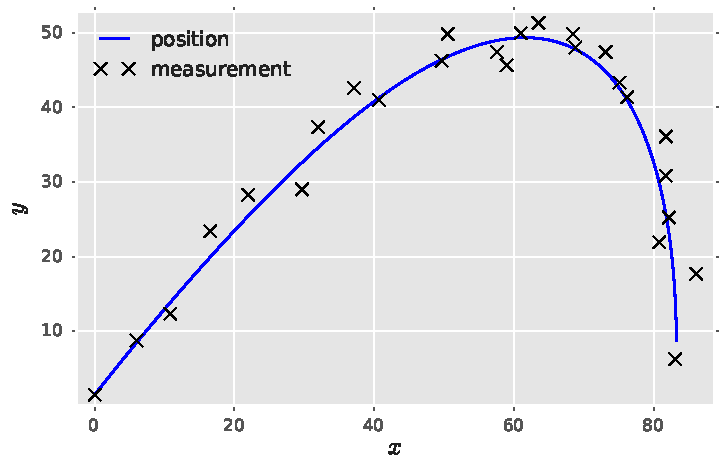
\includegraphics[width=\textwidth]{img/ex1_pos_meas}%
    	\caption{The noisy measurements are plotted with crosses. The initial point is at the origo.}%
		\label{fig:ballistic_flight}%
    \end{subfigure}
    \begin{subfigure}[b]{0.5\textwidth}%
    	%\captionsetup{margin=0pt}
    	\centering%
		\includegraphics[width=\textwidth]{img/ex1_x2}%
    	\caption{$x$ velocity}%
		\label{fig:ballistic_x2}%
    \end{subfigure}%
    \begin{subfigure}[b]{0.5\textwidth}%
    	\centering%
		\includegraphics[width=\textwidth]{img/ex1_x5}%
    	\caption{$y$ velocity}\label{fig:ballistic_x5}%
    \end{subfigure}
	
    \begin{subfigure}[b]{0.5\textwidth}%
    	\centering%
		\includegraphics[width=\textwidth]{img/ex1_x3}%
    	\caption{$x$ acceleration}\label{fig:ballistic_x3}%
    \end{subfigure}%
    \begin{subfigure}[b]{0.5\textwidth}
    	\centering%
		\includegraphics[width=\textwidth]{img/ex1_x6}%
    	\caption{$y$ acceleration}\label{fig:ballistic_x6}%
    \end{subfigure}%
	\caption{A simulation of the the ballistic object in 
	Example~\ref{ex:ballistic}.}
	\label{fig:ballistic}
 \end{figure}
 




%% Leave first page empty
\thispagestyle{empty}


\clearpage

\section{Background}
\subsection{State space models}

State space models (SSMs) provide a unified probabilistic methodology for modeling
sequential data \parencite{ljung1994modeling,durbin2012time,Cappe2005,barber2011bayesian}. Sequential data arise in numerous applications, typically in the form
of time-series measurements \todo{examples}. However it is not necessary for the sequence index to have
a temporal meaning. In probabilistic terms a time-series
can be described by a \emph{stochastic process} $\z = \left\{\z_k:k\in K\right\}$, where $\z_k$ is a random
variable and $K\subset\R$ for continuous time or $K\subset\field{N}$ for discrete time sequences. 
In this thesis we will only be concerned with discerete time processes and the sample space of $\z_k$ will be $\R^d$. 
The shorthand $\z_{1:k}$ will be used to mean the subset $\{\z_1,\dots,\z_k\}$. We will also
denote by $\v{Z}$ the $d\times T$ matrix, that has all $T$ values of the process $\z$ as columns.

A fundamental question in probabilistic models for sequential data is how 
to model the dependence between variables. It is infeasible to assume
that every random variable in the process depends on all the others.
Thus it is common to assume a \emph{Markov chain}, where the distribution of
the process at the current timestep depends only on the distribution in the previous timestep.
A further assumption in SSMs is that the process of interest, the dynamic process $\x$, is not directly observed
but only through another stochastic process, the \emph{measurement process} $\y$. Since
$\x$ is not observed, SSMs belong to the class of \emph{latent variable models}. Sometimes, as in
\cite{Cappe2005}, SSMs are called \emph{hidden Markov models} (HMM) but usually this implies that
the sample space of $\x$ is discrete. Another assumption is that the values of the measurement process are conditionally independent
given the latent Markov process.
An intuitive way to present conditional independence properties between random
variables is a \emph{Bayes network} presented by a directed acyclic graph (DAG) \parencite{pearl1988probabilistic,Bishop2006}.
%The conditional independence properties of a discrete-time SSM are presented in figure~\ref{fig:ssm_graphical}.
A Bayes network presentation of a discrete-time SSM is given in figure~\ref{fig:ssm_graphical}.

\begin{figure}[!htp]
	\centering
	\begin{tikzpicture}
	\tikzstyle{main}=[circle, minimum size = 5mm, inner sep=0mm, thick, draw =black!80, node distance = 12mm,font=\small]
	\tikzstyle{param}=[circle, minimum size = 2mm, inner sep=0mm, thick, draw =white!80, fill=black!80, node distance = 18mm]
	\tikzstyle{ellipsis}=[circle, minimum size = 10mm, thick, draw =black!80, node distance = 18mm]
	\tikzstyle{connect}=[-latex, semithick]
	  %\node[main,node distance=50mm] (theta) [label=above:$\theta$] {};
	  \node[main] (x_1) [label=above:$\v{x}_{k-1}$] {};
	  \node[main,draw=white!0] (prev) [left of=x_1] {$\dots$};
	  \node[main] (x) [right of=x_1,label=above:$\v{x}_{k}$] {};
	  \node[main] (x__1) [right of=x,label=above:$\v{x}_{k+1}$] {};
	  \node[main,fill = black!10] (y_1) [below of=x_1,label=below:$\v{y}_{k-1}$] {};
	  \node[main,fill = black!10] (y) [below of=x,label=below:$\v{y}_{k}$] {};
	  \node[main,fill = black!10] (y__1) [below of=x__1,label=below:$\v{y}_{k+1}$] {};
	  \node[main,draw=white!0] (next) [right of=x__1] {$\dots$};
	  \path
	    (prev) edge [connect] (x_1)
	    (x_1) edge [connect] (x) 
	    	  edge [connect] (y_1)
	    (x) edge [connect] (y)
	    	edge [connect] (x__1)
	    (x__1) edge [connect] (y__1)
	    	edge [connect] (next);
	\end{tikzpicture}
	\caption{SSM as a graphical model presented with a directed acyclic graph}
	\label{fig:ssm_graphical}
\end{figure}
The value $\xk \in \mathcal{X} \subset \R^{d_x}$ of the dynamic process at time $k$ is called the
\emph{state}\todo{Explain state} at time $k$. For the measurements we define $\yk \in \mathcal{Y} \subset \R^{d_y}$.  
Taking into account the Markov property 
\begin{align}
	\Pdf{\xk}{\x_{1:k-1}}&=\Pdf{\xk}{\x_{k-1}}
\end{align}
of the dynamic process and the conditional
independence property 
\begin{align}
	\Pdf{\yk}{\x_{1:k},\y_{1:k-1}}&=\Pdf{\yk}{\xk}
\end{align}
of the measurement process, the joint distribution of states
and measurements factorises as
\begin{align}
	\Pdf{\X,\Y}{\Th}&=\Pdf{\v{x}_0}{\Th}\prod_{k=1}^T\Pdf{\v{x}_k}{\v{x}_{k-1},\Th}\Pdf{\v{y}_k}{\v{x}_{k},\Th}
	\label{eq:complete_data_likelihood}.
\end{align}
Thus in order to describe a SSM one needs to specify three probability distributions:
\begin{description}
\addtolength{\leftskip}{1cm}
	\item[Prior distribution]
	$\Pdf{\v{x}_0}{\Th}$ is the distribution assumed for the state prior to observing any measurements. The
	sensitivity of the posterior distributions to the prior depends on the amount of data (the more data the less sensitivity).
	\item[Dynamic model]
	$\Pdf{\v{x}_k}{\v{x}_{k-1},\Th}$ dictates the time evolution of the states
	\item[Measurement model]
	$\Pdf{\v{y}_k}{\v{x}_{k},\Th}$ models how the observations depend on the state and the statistics of the noise
\end{description}
In this thesis it is assumed that the parametric form of these distributions is known
for example by physical modeling \parencite{ljung1994modeling}. However the distributions are dependent on
the vector parameter $\Th \in \Theta \subset \R^{d_\theta}$ whose value (or distribution) we would like to learn from
the measurements.

Traditionally SSMs are specified as a pair of equations specifying the dynamic and measurement models. The most general
presentation of discrete-time SSMs is 
\begin{subequations}
\label{eq:ssm_too_general}
\begin{align}
	\xk &= \v{f}_{\Th,k}\left(\x_{k-1},\v{q}_{k-1}\right)\\
	\yk &= \v{h}_{\Th,k}\left(\xk,\v{r}_{k}\right).
\end{align}
\end{subequations}
Here the stochasticity is separated into the noise processes $\v{q}$ and $\v{r}$ which are usually
assumed to be zero mean, white and independent of each other. We will restrict ourselves
to the case of zero mean, white and additive Gaussian noise and in our case the mappings
$\v{f}_{\Th,k}$ and $\v{h}_{\Th,k}$ and the noise processes $\v{q}$ and $\v{r}$ will be stationary (i.e. independent of
k). Thus the SSMs considered in this thesis are of the form
\begin{subequations}
\label{eq:ssm_general}
\begin{alignat}{2}
	\xk &= \v{f}_{\Th}\left(\x_{k-1}\right)+\v{q}_{k-1}&\v{q}_k&\sim \N{\v{0},\v{Q}} \label{eq:Q}\\
	\yk &= \v{h}_{\Th}\left(\xk\right)+\v{r}_{k}&\v{r}_k&\sim \N{\v{0},\v{R}} \label{eq:R}\\
	\v{x}_{0} &\sim \N{\gv{\mu},\gv{\Sigma}}& \label{eq:prior}
\end{alignat}
\end{subequations}
We will assume an implicit dependence of the distributional parameters $\v{Q}$,
$\v{R}$,$\gv{\mu}$ and $\gv{\Sigma}$ on $\Th$. 
Now clearly the mappings $\v{f}_{\Th}:\mathcal{X}\to\mathcal{X}$ and
$\v{h}_{\Th}:\mathcal{X}\to\mathcal{Y}$ specify the means of the dynamic
and the measurement models:
\begin{subequations}
\label{eq:ssm_distr_general}
\begin{align}
	\Pdf{\xk}{\x_{k-1},\Th}&=\N{\v{f}_{\Th}\left(\x_{k-1}\right),\v{Q}}\label{eq:dynamics_distr_general}\\
	\Pdf{\yk}{\xk,\Th}&=\N{\v{h}_{\Th}\left(\xk\right),\v{R}}\label{eq:measurement_distr_general}
\end{align}
\end{subequations}

\subsubsection*{Example: 1D random walk}
The simplest example is a one dimensional random-walk observed in Gaussian noise.
We will assume $\Pdf{\v{x}_0}=\N{0,P_0}$. In an alternative (but equivalent) notation
the dynamics model is now
\begin{align}
	\Pdf{x_k}{x_{k-1}}&=x_{k-1}+q_{k-1},
\end{align}
where $q_{k-1}\sim \N{0,Q}$ and the measurement model is
\begin{align}
	\Pdf{y_k}{x_{k}}&=x_{k}+r_{k},
\end{align}
where $r_{k}\sim \N{0,R}$. A simulation from the model is presented in figure~\ref{fig:rw1d}.

\begin{figure}[htp]
\begin{center}
	\missingfigure{A missing 1D RW simulation}
  \caption{Simulation from the 1D RW model}
  \label{fig:rw1d}
\end{center}
\end{figure}


\subsection{Bayesian optimal filtering and smoothing}

Inference can be defined as answering questions of interest with a probability distribution \parencite{barber2011bayesian}.
In case of SSMs there are many questions of interest, but most commonly one would
like to know the \emph{marginal posterior distribution} of the states. State inference
can be divided into subcategories based on the temporal relationship between the state
and the observations \parencite{Sarkka2006}:
\begin{description}
\addtolength{\leftskip}{1cm}
	\item[Predictive distribution]
	$\Pdf{\v{x}_{k}}{\v{y}_{1:k-1}}$ is the predicted distribution of the state in the next timestep (or more generally at timestep $k+h$, where $h>0$) 
	given the previous measurements
	\item[Filtering distribution] $\Pdf{\v{x}_k}{\v{y}_{1:k}}$ is the marginal posterior distribution
	of any state $\xk$ given the measurements up to and including $\yk$
	\item[Smoothing distribution]
	$\Pdf{\v{x}_k}{\v{y}_{1:T}}$ is the marginal posterior distribution
	of any state $\xk$ given the measurements up to and including $\y_T$ where $k<T$
\end{description} 


\subsubsection*{Predictive distribution}
Let us now derive a recursive formulation for computing the filtering distribution at time $k$. Let $\Pdf{\xkk}{\y_{1:k-1}}$
be the filtering distribution of the previous step. Then 
\begin{align}
	\Pdf{\xk}{\y_{1:k-1}}&=\defint{}{}{\Pdf{\xk,\xkk}{\y_{1:k-1}}}{\xkk} \nonumber\\
	&=\defint{}{}{\Pdf{\xk}{\xkk}\Pdf{\xkk}{\y_{1:k-1}}}{\xkk},
	\label{eq:pred_bayes}
\end{align}
which is known as the \emph{Chapman-Kolmogorov equation} \parencite{Sarkka2006}.
\subsubsection*{Filtering distribution}
Incorporating the newest measurement can be achieved with the Bayes'
rule (see for example \cite{gelman2004})\todo{check marginal likelihood wording}
\begin{align}
	\underbrace{\Pdf{\xk}{\y_{1:k}}}_\text{posterior}&=\frac{\overbrace{\Pdf{\yk}{\xk}}^\text{likelihood}\overbrace{\Pdf{\xk}{\y_{1:k-1}}}^\text{prior}}{\underbrace{\Pdf{\y_{k}}{\y_{1:k-1}}}_\text{marginal likelihood}}\nonumber\\
	&=\frac{\Pdf{\yk}{\xk}\Pdf{\xk}{\y_{1:k-1}}}{\defint{}{}{\Pdf{\yk}{\xk}\Pdf{\xk}{\y_{1:k-1}}}{\xk}}
\end{align}
which is called the measurement update equation.

\subsubsection*{Smoothing distribution}
The smoothing distributions can also be computed recursively by assuming that the filtering distributions
and the smoothing distribution $\Pdf{\x_{k+1}}{\y_{1:T}}$ of the ``previous'' step are available.
Since
\begin{align*}
	\Pdf{\xk}{\x_{k+1},\y_{1:T}}&=\Pdf{\xk}{\x_{k+1},\y_{1:k}}\\
	&=\frac{\Pdf{\xk,\x_{k+1}}{\y_{1:k}}}{\Pdf{\x_{k+1}}{\y_{1:k}}}\\
	&=\frac{\Pdf{\x_{k+1}}{\xk}\Pdf{\xk}{\y_{1:k}}}{\Pdf{\x_{k+1}}{\y_{1:k}}}
\end{align*}
we get
\begin{align}
	\Pdf{\xk}{\y_{1:T}}&=\Pdf{\xk}{\y_{1:k}}\defint{}{}{\left[\frac{\Pdf{\x_{k+1}}{\xk}\Pdf{\x_{k+1}}{\y_{1:T}}}{\Pdf{\x_{k+1}}{\y_{1:k}}}\right]}{\x_{k+1}},
\end{align}
where $\Pdf{\x_{k+1}}{\y_{1:k}}$ can be computed by equation \eqref{eq:pred_bayes}.

\subsubsection*{Marginal likelihood}

An important quantity concerning parameter estimation is the marginal likelihood $\Pdf{\y_{1:T}}$. Since
\begin{align}
	\Pdf{\y_k}{\y_{1:k-1}}&=\defint{}{}{\Pdf{\yk}{\xk}\Pdf{\xk}{\y_{1:k-1}}}{\xk}
\end{align}
the marginal likelihood can be computed from
\begin{align}
	\Pdf{\y_{1:T}}&=\Pdf{\y_1}\prod_{k=2}^T \Pdf{\y_k}{\y_{1:k-1}}
\end{align}






\section{State estimationin SSMs}
\subsection{Linear-Gaussian State Space Models}

Linear-Gaussian SSMs can be defined with the following equations
\begin{subequations}
	\label{eq:the_model}
	\begin{align}
		\v{x}_k&=\v{A}\v{x}_{k-1}+\v{q}_{k-1} \label{eq:dynamics}\\
		\v{y}_k&=\v{H}\v{x_k}+\v{r}_k \label{eq:measurements}\\
		\v{q}_{k-1} &\sim \N{0,\v{Q}} \label{eq:pdf_dynamic_noise}\\
		\v{r}_{k} &\sim \N{0,\v{R}} \label{eq:pdf_measurement_noise}\\
		\v{x}_{0} &\sim \N{\gv{\mu},\gv{\Sigma}}
	\end{align}
\end{subequations}
Equations \eqref{eq:dynamics}, \eqref{eq:measurements}, \eqref{eq:pdf_dynamic_noise} and \eqref{eq:pdf_measurement_noise}
together specify the following conditional distributions
\begin{align}
		\v{x}_{k}|\v{x}_{k-1} &\sim \N{\v{A}\v{x}_{k-1},\v{Q}} \label{eq:pdf_xk_xk-1}\\
		\v{y}_{k}|\v{x}_{k} &\sim \N{\v{H}\v{x_k},\v{R}}  \label{eq:pdf_yk_xk}
\end{align}

Linearity in this case means that $\v{x}_k$ is a linear combination\todo{Better wording}
of the elements of $\v{x}_{k-1}$ and $\v{y}_k$ is a linear combination
of the elements of $\v{x}_{k}$ (with additive noise in both cases). Since
the noise terms $\v{q}_{k-1}$ and $\v{r}_{k}$ are assumed to be white and
Gaussian, these models are called linear-Gaussian.

\subsubsection{Kalman filter}

To derive the expression for the log-likelihood function in our case,
let us first see what the Kalman filter calculates. Firstly,
the recursions are as follows \parencite{Mbalawataa}:
\begin{subequations}
\begin{align}
	\shortintertext{prediction:}
	\v{m}_{k|k-1}&=\v{A}\v{m}_{k-1|k-1}\\
	\v{P}_{k|k-1}&=\v{A}\v{P}_{k-1|k-1}\v{A}^T+\v{Q}
	\shortintertext{update:}
	\v{v}_k&=\v{y}_k-\v{H}\v{m}_{k|k-1}\\
	\v{S}_k&=\v{H}\v{P}_{k|k-1}\v{H}^T+\v{R}\\
	\v{K}_k&=\v{P}_{k|k-1}\v{H}^T\v{S}_{k}^{-1}\\
	\v{m}_{k|k}&=\v{m}_{k|k-1}+\v{K}_k\v{v}_k\\
	\v{P}_{k|k}&=\v{P}_{k|k-1}-\v{K}_k\v{S}_k\v{K}_{k}^T
\end{align}
\end{subequations}
This includes the sufficient statistics for the $T$
joint distributions 
\begin{align}
\begin{split}
	\Pdf{\v{x}_k,\v{y}_k}{\v{y}_1,\dots,\v{y}_{k-1},\gv{\theta}}
	&=N\left(
	\begin{bmatrix}
		\v{x}_k\\\v{y}_{k}
	\end{bmatrix}\left\vert
	\begin{bmatrix}
		\v{m}_{k|k-1}\\
		\v{H}\v{m}_{k|k-1}
	\end{bmatrix}
	\right.,
	\begin{bmatrix}
		\v{P}_{k|k-1} & \v{P}_{k|k-1}\v{H}^T\\
		\v{H}\v{P}_{k|k-1}^T & \v{S}_k  
	\end{bmatrix}
	\right)\\
	\Rightarrow \Pdf{\v{y}_k}{\v{y}_1,\dots,\v{y}_{k-1},\gv{\theta}}
	&=N\left(\cond{\v{y}_k}{\v{H}\v{m}_{k|k-1},\v{S}_k }\right)
\end{split}
	\label{eq:joint_per_kalmanstep}
\end{align}

\subsubsection{RTS Smoother}

The standard RTS smoother gives the statistics $\v{m}_{k|N}$ and $\v{P}_{k|N}$.
The cross-timestep variance $\v{C}_{k|N}$ can be computed with an additional
recursive formula alongside the usual RTS smoother recursions
\begin{subequations}
\begin{align}
	\v{J}_k&=\v{P}_{k|k}\v{A}^T\v{P}_{k|k+1}^{-1}\\
	\v{m}_{k|N}&=\v{m}_{k|k}+\v{J}_k\left(\v{m}_{k+1|N}-\v{m}_{k+1|k}\right)\\
	\v{P}_{k|N}&=\v{P}_{k|k}+\v{J}_k\left(\v{P}_{k+1|N}-\v{P}_{k+1|k}\right)\v{J}_k^T\\
	\v{C}_{k|N}&=\v{P}_{k|k}\v{J}_{k-1}^T+\v{J}_k\left(\v{C}_{k+1|N}-\v{A}\v{P}_{k|k}\right)\v{J}_{k-1}^T\\
\end{align}
\end{subequations}
For more specific details see \parencite{Gibson2005}. All in all, the E-step of the 
EM algorithm in linear-Gaussian SSM:s corresponds to computing
the matrices in \eqref{eq:sum_expectations} with the help of the Kalman filter and
the RTS smoother. In \parencite{Elliott1999} a new kind of filter is presented that
can compute \eqref{eq:sum_expectations} with only forward recursions. 

\subsection{Nonlinear-Gaussian SSMs}

The SSM model is now
\begin{subequations}
	\label{eq:the_model}
	\begin{align}
		\v{x}_k&=\v{f}(\v{x}_{k-1})+\v{q}_{k-1} \label{eq:dynamics_nonlinear}\\
		\v{y}_k&=\v{h}(\v{x_k})+\v{r}_k \label{eq:measurements_nonlinear}\\
		\v{q}_{k-1} &\sim \N{0,\v{Q}} \label{eq:pdf_dynamic_noise_nonlinear}\\
		\v{r}_{k} &\sim \N{0,\v{R}} \label{eq:pdf_measurement_noise_nonlinear}\\
		\v{x}_{0} &\sim \N{\gv{\mu},\gv{\Sigma}}
	\end{align}
\end{subequations}
We assume an implicit dependence of $f$ and $h$ on the parameter $\Th$.

\subsubsection{Assumed density filtering and smoothing}


One approach to forming Gaussian approximations is to assume a
Gaussian probability density function with mean and variance that match the
actual ones. Let 

\begin{align}
	\v{a}&\sim \N{\v{m},\gv{\Sigma}_a} \label{eq:pa}\\
	\v{b}|\v{a}&\sim \N{\v{f}(\v{a}),\gv{\Sigma}_{b|a}} \label{eq:pb_given_a}
\end{align}
then 
\begin{align}
	\label{eq:joint_nongaussian}
	\Pdf{\v{a},\v{b}}&=\N{\v{m},\gv{\Sigma}_a}\N{\v{f}(\v{a}),\gv{\Sigma}_{b|a}}
\end{align}
is only Gaussian if $\v{f}(\v{a})$ is linear. Let the Gaussian approximation
to \eqref{eq:joint_nongaussian} be

\begin{align}
	\label{eq:joint_gaussian_approx}
	\Pdf{\begin{bmatrix}
		\v{a}\\
		\v{b}
	\end{bmatrix}}&\approx
	\N{
	\begin{bmatrix}
		\gv{\mu}_a\\
		\gv{\mu}_b
	\end{bmatrix},
	\begin{bmatrix}
		\gv{\Sigma}_{aa}&\gv{\Sigma}_{ab}\\
		\gv{\Sigma}_{ba}&\gv{\Sigma}_{bb}
	\end{bmatrix}
	}
\end{align}
Then since the marginal distributions of a Gaussian distribution are also
Gaussian, we have to have
\begin{align}
	\gv{\mu}_a&=\v{m}\\
	\gv{\Sigma}_{aa}&=\gv{\Sigma}_{a}\\
	\gv{\mu}_b&=\defint{}{}{\v{b}\Pdf{\v{b}}}{\v{b}} \label{eq:mub}\\
	\gv{\Sigma}_{bb}&=\defint{}{}{(\v{b}-\gv{\mu}_b)(\v{b}-\gv{\mu}_b)^T\Pdf{\v{b}}}{\v{b}} \label{eq:varb}
\end{align}
Both \eqref{eq:mub} and \eqref{eq:varb} can be written in terms of \eqref{eq:pa} and \eqref{eq:pb_given_a}.
To see this, let us rewrite \eqref{eq:mub} as
\begin{align}
	\gv{\mu}_b&=\defint{}{}{\v{b}\Pdf{\v{b}}}{\v{b}} \nonumber\\
	&=\defint{}{}{\v{b}\defint{}{}{\Pdf{\v{b}}{\v{a}}\Pdf{\v{a}}}{\v{a}}}{\v{b}}\nonumber\\
	&=\defint{}{}{\defint{}{}{\v{b}\Pdf{\v{b}}{\v{a}}}{\v{b}}\Pdf{\v{a}}}{\v{a}}\nonumber\\
	&=\defint{}{}{\v{f}(\v{a})\N{\v{m},\gv{\Sigma}_a}}{\v{a}}\label{eq:mean_int}
\end{align}
and \eqref{eq:varb} as
\begin{align}
	\gv{\Sigma}_{bb}&=\defint{}{}{\v{b}\v{b}^T\Pdf{\v{b}}}{\v{b}}-\gv{\mu}_b\gv{\mu}_b^T \nonumber\\
	%&=\defint{}{}{\defint{}{}{\lbrack(\v{b}-\v{f}(\v{a}))(\v{b}-\v{f}(\v{a}))^T+\v{f}(\v{a})\v{f}(\v{a})^T\rbrack\Pdf{\v{b}}{\v{a}}}{\v{b}}\Pdf{\v{a}}}{\v{a}}-\gv{\mu}_b\gv{\mu}_b^T\\
	\begin{split}
	&=\defint{}{}{\v{f}(\v{a})\v{f}(\v{a})^T\Pdf{\v{a}}}{\v{a}}-\gv{\mu}_b\gv{\mu}_b^T\\
	&\qquad+\defint{}{}{\defint{}{}{\lbrack(\v{b}-\v{f}(\v{a}))(\v{b}-\v{f}(\v{a}))^T\rbrack\Pdf{\v{b}}{\v{a}}}{\v{b}}\Pdf{\v{a}}}{\v{a}}
	\end{split}\nonumber\\
	&=\defint{}{}{(\v{f}(\v{a})-\gv{\mu}_b)(\v{f}(\v{a})-\gv{\mu}_b)^T\N{\v{m},\gv{\Sigma}_a}}{\v{a}}+\gv{\Sigma}_{b|a}\label{eq:var_int}.
\end{align}
Finally, the cross-covariance $\gv{\Sigma}_{ab}=\gv{\Sigma}_{ba}^T$ similarly reads
\begin{align}
	\gv{\Sigma}_{ab}&=\defint{}{}{\defint{}{}{(\v{a}-\gv{\mu}_a)(\v{b}-\gv{\mu}_b)^T\Pdf{\v{a},\v{b}}}{\v{a}}}{\v{b}} \nonumber\\
	&=\defint{}{}{\defint{}{}{(\v{a}-\gv{\mu}_a)(\v{b}-\gv{\mu}_b)^T\Pdf{\v{a}}\Pdf{\v{b}}{\v{a}}}{\v{a}}}{\v{b}} \nonumber\\
	&=\defint{}{}{(\v{a}-\gv{\mu}_a)(\defint{}{}{\v{b}\Pdf{\v{b}}{\v{a}}}{\v{b}}-\gv{\mu}_b)^T\Pdf{\v{a}}}{\v{a}} \nonumber\\
	&=\defint{}{}{(\v{a}-\v{m})(\v{f}(\v{a})-\gv{\mu}_b)^T\N{\v{m},\gv{\Sigma}_a}}{\v{a}}\label{eq:cross_cov_int}
\end{align}


 
To see how this idea can be used to form a Gaussian
approximation to \eqref{eq:joint_posterior_of_consecutive_states}, let us
rewrite \eqref{eq:joint_posterior_of_consecutive_states} as
\begin{align}
\begin{split}
	\Pdf{\v{x}_{k-1},\v{x}_{k}}{\v{Y}}&=\Pdf{\v{x}_{k-1}}{\v{x}_{k},\v{Y}_{1:k-1}}\Pdf{\v{x}_{k}}{\v{Y}}\\
	&=\frac{\Pdf{\v{x}_{k-1},\v{x}_{k}}{\v{Y}_{1:k-1}}\Pdf{\v{x}_{k}}{\v{Y}}}{\Pdf{\v{x}_{k}}{\v{Y}_{1:k-1}}},
	\label{eq:joint_smooth}
\end{split}
\end{align}
where the dependance on the current estimate of the parameter $\hat{\Th}_j$
is suppressed for clarity. Since the Gaussian approximation to
\eqref{eq:joint_posterior_of_consecutive_states} will be calculated by forward
(filtering) and backward (smoothing) recursions, let us assume that we already
have available the Gaussian approximation

\begin{align}
	%\Pdf{\v{x}_{k}}{\v{Y},\hat{\Th}_j} &\approx \N{\v{m}_{k|N},\v{P}_{k|N}}\\
	\Pdf{\v{x}_{k-1}}{\v{Y}_{1:k-1},\hat{\Th}_j} &\approx \N{\v{m}_{k-1|k-1},\v{P}_{k-1|k-1}}.
	%\Pdf{\v{x}_{k}}{\v{Y}_{1:k-1},\hat{\Th}_j} &\approx \N{\v{m}_{k|k-1},\v{P}_{k|k-1}}.
\end{align}
The Gaussian approximation to 
\begin{align}
\Pdf{\v{x}_{k-1},\v{x}_{k}}{\v{Y}_{1:k-1}}=\N{\v{x}_{k}}{\v{f}(\v{x}_{k-1}),\v{Q}}\Pdf{\v{x}_{k-1}}{\v{Y}_{1:k-1}}
\end{align}
is then given by application of equations \eqref{eq:mean_int}, \eqref{eq:var_int} and \eqref{eq:cross_cov_int} 
\begin{align}
	\begin{split}
	\v{m}_{k|k-1}&=\defint{}{}{\v{f}(\v{x}_{k-1})\N{\v{x}_{k-1}}{\v{m}_{k-1|k-1},\v{P}_{k-1|k-1}}}{\v{x}_{k-1}}\label{eq:prediction_mean_intergral}
	\end{split}\\
	\begin{split}
	\v{P}_{k|k-1}&=\defint{}{}{(\v{f}(\v{x}_{k-1})-\v{m}_{k|k-1})(\v{f}(\v{x}_{k-1})-\v{m}_{k|k-1})^T\\
	&\qquad\N{\v{x}_{k-1}}{\v{m}_{k-1|k-1},\v{P}_{k-1|k-1}}}{\v{x}_{k-1}}+\v{Q}\label{eq:prediction_variance_intergral}
	\end{split}\\
	\begin{split}
		\v{C}_{k^-}&=\defint{}{}{(\v{x}_{k-1}-\v{m}_{k-1|k-1})(\v{f}(\v{x}_{k-1})-\v{m}_{k|k-1})^T\\
		&\qquad\N{\v{x}_{k-1}}{\v{m}_{k-1|N},\v{P}_{k-1|N}}}{\v{x}_{k-1}}\label{eq:prediction_cov_intergral}
	\end{split}
\end{align}
so that the approximation is
\begin{align}
	\Pdf{\v{x}_{k-1},\v{x}_k}{\v{Y}_{1:k-1},\hat{\Th}_j}&\approx 
	\N{
	\begin{bmatrix}
		\v{m}_{k-1|k-1}\\
		\v{m}_{k|k-1}
	\end{bmatrix},
	\begin{bmatrix}
		\v{P}_{k-1|k-1}&\v{C}_{k^-}\\
		\v{C}_{k^-}^T&\v{P}_{k|k-1}
	\end{bmatrix}
	}
	\label{eq:joint_predictive_approximation}
\end{align}
In order to calculate \eqref{eq:prediction_mean_intergral} and \eqref{eq:prediction_variance_intergral}
we also need a Gaussian approximation for the joint distribution of
the current state and measurement given the previous measurements
\begin{align}
\begin{split}
	\Pdf{\v{x}_{k},\v{y}_k}{\v{Y}_{1:k-1}}&=\N{\v{y}_{k}}{\v{h}(\v{x}_{k}),\v{R}}\Pdf{\v{x}_{k}}{\v{Y}_{1:k-1}}\\
	&\approx 
	\N{
	\begin{bmatrix}
		\v{m}_{k|k-1}\\
		\gv{\mu}_{k}
	\end{bmatrix},
	\begin{bmatrix}
		\v{P}_{k|k-1}&\v{C}_{k}\\
		\v{C}_{k}^T&\v{S}_{k}
	\end{bmatrix}
	}.
	\label{eq:joint_update_approximation}
\end{split}
\end{align}
Applying equations \eqref{eq:mean_int}, \eqref{eq:var_int} and \eqref{eq:cross_cov_int} again,
we get
\begin{align}
	\gv{\mu}_{k}
	&=\defint{}{}{\v{h}(\v{x}_{k})\N{\v{x}_{k}}{\v{m}_{k|k-1},\v{P}_{k|k-1}}}{\v{x}_{k}}\label{eq:update_mean_intergral}\\
	\v{S}_{k}
	&=\defint{}{}{(\v{h}(\v{x}_{k})-\gv{\mu}_k)(\v{h}(\v{x}_{k})-\gv{\mu}_k)^T\N{\v{x}_{k}}{\v{m}_{k|k-1},\v{P}_{k|k-1}}}{\v{x}_{k}}+\v{R} \label{eq:update_variance_intergral}\\
	\v{C}_{k}
	&=\defint{}{}{(\v{x}_{k}-\v{m}_{k|k-1})(\v{h}(\v{x}_{k})-\gv{\mu}_k)^T\N{\v{x}_{k}}{\v{m}_{k|k-1},\v{P}_{k|k-1}}}{\v{x}_{k}} \label{eq:update_covariance_intergral}
\end{align}
and by using the well known formula for calculating the conditional distribution of jointly Gaussian variables
we have
\begin{align}
	\v{m}_{k|k}
	&=\v{m}_{k|k-1}+\v{C}_{k}\v{S}_{k}^{-1}\left(\v{y}_k-\gv{\mu}_k\right)\label{eq:update_mean}\\
	\v{P}_{k|k}
	&=\v{P}_{k|k-1}-\v{C}_{k}\v{S}_{k}^{-1}\v{C}_{k}^T. \label{eq:update_variance}
\end{align}
Again using the formula for the conditional of jointly Gaussian variables we get
from \eqref{eq:joint_predictive_approximation}
\begin{align}
	\Pdf{\v{x}_{k-1}}{\v{x}_k,\v{Y}_{1:k-1}}&\approx\N{\v{m}_2,\v{P}_2}\\
	\v{G}_{k-1}&=\v{C}_{k^-}\v{P}_{k|k-1}^{-1}\\
	\v{m}_2&=\v{m}_{k-1|k-1}+\v{G}_{k-1}(\v{x}_k-\v{m}_{k|k-1})\\
	\v{P}_2&=\v{P}_{k-1|k-1}-\v{G}_{k-1}\v{P}_{k|k-1}\v{G}_{k-1}^T
\end{align}
and then finally we can write the Gaussian approximation to the joint distribution of consecutive states given all the measurements
as
\begin{align}
\begin{split}
	\Pdf{\v{x}_{k-1},\v{x}_{k}}{\v{Y}}&=\Pdf{\v{x}_{k-1}}{\v{x}_{k},\v{Y}_{1:k-1}}\Pdf{\v{x}_{k}}{\v{Y}}\\
	&\approx
	\N{
	\begin{bmatrix}
		\v{m}_{k-1|N}\\
		\v{m}_{k|N}
	\end{bmatrix},
	\begin{bmatrix}
		\v{P}_{k-1|N}&\v{D}_{k}\\
		\v{D}_{k}^T&\v{P}_{k|N}
	\end{bmatrix}
	}
\end{split}
\end{align}
where
\begin{align}
	\v{D}_{k}&=\v{G}_{k-1}\v{P}_{k|N}\\
	\v{m}_{k-1|N}&=\v{m}_{k-1|k-1}+\v{G}_{k-1}\left(\v{m}_{k|N}-\v{m}_{k|k-1}\right)\\
	\v{P}_{k-1|N}&=\v{P}_{k-1|k-1}+\v{G}_{k-1}\left(\v{P}_{k|N}-\v{P}_{k|k-1}\right)\v{G}_{k-1}^T
\end{align}

\subsubsection{Quadrature and Cubature}
\subsubsection{Gauss-Hermite Kalman Filter and Smoother}
\subsubsection{Unscented Kalman Filter and Smoother}
\subsubsection{Cubature Kalman Filter and Smoother}





\section{Parameter estimation in SSMs}
%%%%%%%%%%%%%%%%%%%%%%%%%%%%%%%%%%%%%%%%%%%%%%%%%%%%%%%%%%%%%%%%%%%%%%%%%
\subsection{Maximum likelihood and maximum a posteriori estimation}%%%%%%
%%%%%%%%%%%%%%%%%%%%%%%%%%%%%%%%%%%%%%%%%%%%%%%%%%%%%%%%%%%%%%%%%%%%%%%%%

In the Bayesian sense the complete answer to the parameter estimation
problem is the marginal posterior probability of the parameters
given the measurements, which is given by Bayes' rule as
\begin{align}
	\Pdf{\gv{\theta}}{\Y}&=\frac{\Pdf{\Y}{\gv{\theta}}\Pdf{\gv{\theta}}}{\Pdf{\Y}}.
	\label{eq:param_post}
\end{align}

Computing the posterior distribution of the parameters is usually intractable \todo{why? examples?}. A much
easier problem is finding a suitable \emph{point estimate} $\hat{\gv{\theta}}$.
This effectively means that we don't need to worry about the normalizing
term $\Pdf{\Y}$, since it's constant with respect to the parameters. 
A point estimate that maximizes the posterior distribution
is called a \emph{maximum a posteriori} (MAP) estimate. 
Since the logarithm is a strictly monotonic function, maximizing a function
is the same as maximizing its logarithm. Thus the MAP estimate $\Th^*$ is given by 
\begin{align}
	\Th_{\text{MAP}} &= \text{argmax}_{\Th}\left[\underbrace{\log \Pdf{\Y}{\gv{\theta}}}_{\Pdf[\ell][2pt]{\Th}} + \log\Pdf{\gv{\theta}}\right]
	\label{eq:MAP}
\end{align}

In the case of a flat (constant and thus improper)
prior distribution, $\Pdf{\Th}$, the MAP estimate converges to the
\emph{maximum likelihood} (ML) estimate
\begin{align}
	\Th_{\text{ML}} &= \text{argmax}_{\Th}\left[\lLH\right]
	\label{eq:ML}
\end{align}
Going further we we will only be concerned with finding the ML estimate, but it should
be remembered that both of the methods we consider can be extended
to the estimation of the MAP estimate in a straightforward fashion.
\todo{Explain MAP in both cases}

Among different point estimates, the maximum likelihood estimator has good statistical properties.
Let us denote the true parameter value, the value that the data was generated with, with $\Th_\star$ and 
let $T$ denote the amount of observations.
Then provided that some conditions of not very restricting nature hold, we can state the following asymptotic properties 
for the ML estimate $\Th_{\text{ML}}$:\todo{Modify to reflect p.465 in Cappé}
\begin{description}
\addtolength{\leftskip}{1cm}
\item[Strong consistency]\hfill\\
An important property for an estimator, which says that
the estimator tends to the true value as the amount of data tends to infinity:
\begin{align}
	%\forall \Th \in \Theta\quad \frac{1}{n}\Pdf[\ell_n]{\Th} \xrightarrow{\mathrm{a.s.}} \lLH, \mathrm{when} n\to\infty
	\ell_T\left(\Th_{\text{ML}}\right) \xrightarrow{\mathrm{a.s.}} \ell\left(\Th_\star\right),\quad \mathrm{when}\;T\to\infty,
\end{align}
where $\ell_T$ is the likelihood function after $T$ measurements and $\ell$ is a continuous
deterministic function with a unique global maximum at $\Th_\star$.
%where $\Pdf[\ell_n]{\Th}$ is the log-likelihood given $n$ observations and $\lLH$ is a continuous deterministic
%function with a unique global maximum at $\Th_\star$.
\item[Asymptotic normality]\hfill\\
This property gives us the means to compute asymptotic error bounds for
the estimate:
\begin{align}
	\sqrt{T}\left(\Th_{\text{ML}}-\Th_\star\right) \xrightarrow{D} \N{\v{0},\mathcal{I}^{-1}\left(\Th_\star\right)},\quad \mathrm{when}\;T\to\infty,
	\label{tablelabel}
\end{align}
where $\mathcal{I}\left(\Th_\star\right)$ is the \emph{Fischer information matrix} evaluated at $\Th_\star$ 
\item[Efficiency]\hfill\\
When the amount of information tends to infinity, the ML-estimate achieves
the Cramér-Rao lower bound, i.e. no other consistent estimator has lower asymptotic mean-squared-error.
\end{description}


\subsubsection{Identifiability}

Intuitively, any parameters $\Th,\:\Th' \in \Theta$ cannot be distinguished
from each other with maximum likelihood estimation if
\begin{align}
	\Pdf{\Y}{\Th}&=\Pdf{\Y}{\Th'},
\end{align}
i.e., if the same data can arise with two (or more) separate
parameter values.
\todo{Elaborate on identifiability}
\parencite{Haykin2001,Cappe2005}

%%%%%%%%%%%%%%%%%%%%%%%%%%%%%%%%%%%%%%%%%%%%%%%%%%%%%%%%%%%%%%%%%%%%%
\subsection{Gradient based nonlinear optimization}\label{sec:grad}%%%
%%%%%%%%%%%%%%%%%%%%%%%%%%%%%%%%%%%%%%%%%%%%%%%%%%%%%%%%%%%%%%%%%%%%%

This is the classical way of solving the parameter estimation problem. It consists
of computing the gradient of the log-likelihood function $\lLH$ and then using some
non-linear optimization method to find a \emph{local} maximum to it 
\parencite{Mbalawataa,Cappe2005}. 
An efficient non-linear optimization algorithm is the scaled 
conjugate gradient method \parencite{Mbalawataa}.

By marginalizing the joint distribution of equation~\eqref{eq:joint_per_kalmanstep}
we get 
\begin{align}
	\Pdf{\y_k}{\y_{1:k-1},\Th}&=\N[\yk]{\v{H}\m_{k|k-1},\v{S}_k }.
\end{align}
Applying equation~\eqref{eq:lh_factorization} and taking the logarithm then gives
\begin{align}
	\lLH&=-\frac{1}{2}\sum_{k=1}^N\log\abbs{\v{S}_k}
	-\frac{1}{2}\sum_{k=1}^N\left(\v{y}_k-\v{H}\v{m}_{k|k-1}\right)^T\v{S}_{k}^{-1}\left(\v{y}_k-\v{H}\v{m}_{k|k-1}\right)+C,
	\label{eq:logLH}
\end{align}
where $C$ is a constant that doesn't depend on $\gv{\theta}$ and thus can
be ignored in the maximization.
Employing an efficient numerical optimization method generally
requires that the gradient of the objective function is available. 
There are at least two seemingly quite different methods for computing
the gradient of $\lLH$. The first one proceeds straightforwardly by taking the
partial derivatives of $\lLH$. As will soon be demonstrated, this leads
to some additional recursive formulas which allow computing
the gradient in parallel with the Kalman filter. The second method needs
the smoothing distributions with the cross-timestep covariances of equation~\eqref{eq:rts_cross_timestep_covariance}
and it can be easily computed with the expectation maximization machinery
that will be introduced later. These two methods can be proved to compute
the exact same quantity. At this point we will focus on the first one. 

In order to calculate the gradient of $\lLH$, we can take the partial
derivatives of it w.r.t every parameter $\theta_i$ in $\gv{\theta}$:

\begin{align}
\begin{split}
	\dpd{\lLH}{\theta_i}
	=&-\frac{1}{2}\sum_{k=1}^N\mathrm{Tr}\left(\v{S}_{k}^{-1}\dpd{\v{S}_k}{\theta_i}\right)\\
	&+\sum_{k=1}^N\left(\v{H}_k\dpd{\v{m}_{k|k-1}}{\theta_i}\right)^T\v{S}_{k}^{-1}\left(\v{y}_k-\v{H}\v{m}_{k|k-1}\right)\\
	&+\frac{1}{2}\sum_{k=1}^N\left(\v{y}_k-\v{H}\v{m}_{k|k-1}\right)^T\v{S}_{k}^{-1}\left(\dpd{\v{S}_k}{\theta_i}\right)\v{S}_{k}^{-1}\left(\v{y}_k-\v{H}\v{m}_{k|k-1}\right)\\
	\label{eq:dlogLH}
\end{split}
\end{align}
From the Kalman filter recursions \eqref{eq:Kalman_filter} we find out that 
\begin{align}
	\dpd{\v{S}_k}{\theta_i}&=\v{H}\dpd{\v{P}_{k|k-1}}{\theta_i}\v{H}+\dpd{\v{R}}{\theta_i}
\end{align}
so that we're left with the task of determining the partial derivatives for
$\v{m}_{k|k-1}$ and $\v{P}_{k|k-1}$:

\begin{align}
	\dpd{\v{m}_{k|k-1}}{\theta_i}&=\dpd{\v{A}}{\theta_i}\v{m}_{k-1|k-1}+\v{A}\dpd{\v{m}_{k-1|k-1}}{\theta_i} \label{eq:m_pred_pd}\\
	\begin{split}
	\dpd{\v{P}_{k|k-1}}{\theta_i}&=\dpd{\v{A}}{\theta_i}\v{P}_{k-1|k-1}\v{A}^T+\v{A}\dpd{\v{P}_{k-1|k-1}}{\theta_i}\v{A}^T\\
	&+\v{A}\v{P}_{k-1|k-1}\left(\dpd{\v{A}}{\theta_i}\right)^T+\dpd{\v{Q}}{\theta_i} \label{eq:P_pred_pd}
	\end{split}
\end{align}
as well as for $\v{m}_{k|k}$ and $\v{P}_{k|k}$:
\begin{align}
	\dpd{\v{K}_k}{\theta_i}&=\dpd{\v{P}_{k|k-1}}{\theta_i}\v{H}^T\v{S}_{k}^{-1}-\v{P}_{k|k-1}\v{H}^T\v{S}_{k}^{-1}\dpd{\v{S}_k}{\theta_i}\v{S}_{k}^{-1}
	\label{eq:K_pd}\\
	\dpd{\v{m}_{k|k}}{\theta_i}&=\dpd{\v{m}_{k|k-1}}{\theta_i}+\dpd{\v{K}_k}{\theta_i}\left(\v{y}_k-\v{H}\v{m}_{k|k-1}\right)-\v{K}_k\v{H}\dpd{\v{m}_{k|k-1}}{\theta_i}
	\label{eq:m_pd}\\
	\dpd{\v{P}_{k|k}}{\theta_i}&=\dpd{\v{P}_{k|k-1}}{\theta_i}-\dpd{\v{K}_k}{\theta_i}\v{S}_{k}\v{K}_{k}^T-\v{K}_{k}\dpd{\v{S}_k}{\theta_i}\v{K}_{k}^T-\v{K}_{k}^T\v{S}_{k}\left(\dpd{\v{K}_k}{\theta_i}\right)^T
	\label{eq:P_pd}
	\end{align}
Equations \eqref{eq:m_pred_pd}, \eqref{eq:P_pred_pd}, \eqref{eq:K_pd}, \eqref{eq:m_pd} and \eqref{eq:P_pd} together specify
a recursive algorithm for computing \eqref{eq:dlogLH} that can be run alongside the Kalman filter recursions.
As noted in \textcite{Cappe2005}, these equations are sometimes known as the \emph{sensitivity equations}
and they are derived at least in \textcite{Gupta1974} and \textcite{Mbalawataa}.
\todo{Elaborate on nonlinear programming}  

%%%%%%%%%%%%%%%%%%%%%%%%%%%%%%%%%%%%%%%%%%%%%%
\subsection{Expectation maximization (EM)}%%%%
%%%%%%%%%%%%%%%%%%%%%%%%%%%%%%%%%%%%%%%%%%%%%%

The expectation maximization (EM) algorithm \parencite{Dempster1977} is a general
method for finding ML and MAP estimates in probabilistic models with missing data or
latent variables \parencite{Bishop2006,barber2012bayesian}. As will be seen, instead of maximizing
\eqref{eq:logLH} directly, EM alternates between forming a variational lower bound and maximizing it.
We shall use $\E{\cdot}{q}\equiv\defint{}{}{\cdot \Pdf[q]{z}}{z}$ to denote the expectation
over some arbitrary distribution $\Pdf[q]{z}$.
Let us introduce a ``variational'' 
distribution $\tPX$ over the states, parameterized with $\Th'$ (not necessarily related to $\Th$).
Noting now that $\Pdf{\X}{\Y,\Th}=\cLH/\LH$ and that $\lLH\equiv\log\LH$ is independent of $\X$ we can then perform the
following decomposition on the log likelihood:
\begin{align}
	\lLH &= \log\cLH - \log\post \nonumber\\
	&= \E{\log\cLH}_{\tP} - \E{\log\post}_{\tP} \nonumber\\
	&= \underbrace{\E{\log\cLH-\log\tPX}_{\tP}}_{\LB[1pt]{\tP,\Th}}
	\underbrace{-\E{\log\post-\log\tPX}_{\tP}}_{\KL{\tP}{\post[1pt]}}
	\label{eq:lLH_decomp}
\end{align}
The important step here is taking the expectation over $\tPX$, since the \emph{complete-data log-likelihood}
$\log\cLH$ cannot be evaluated as $\X$ is unobserved.
Since $\KL{\tP}{\post}$, the \emph{Kullback-Leibler divergence} between $\tPX$ and $\post$, is always nonnegative,
we see that 
\begin{align}
	\lLH&\geq \LB{\tP,\Th} \label{eq:em_lh_lb}
\end{align}
with equality when 
\begin{align}
	\tPX &= \post, \label{eq:em_maxq}
\end{align}
i.e. the posterior distribution of the states with equal parameter value $\Th'=\Th$. Considered as a functional
of only $\tP$, clearly $\LB{\tP,\Th}$ is maximized
and $\KL{\tP}{\post}$ vanishes by \eqref{eq:em_maxq}. 
The nonnegativeness of the Kullback-Leibler divergence can be proved by
noting that $-\log$ is a convex function and so \emph{Jensen's inequality}
can be applied \parencite{Bishop2006}.

Let us take a closer at the the first term in \eqref{eq:lLH_decomp} with $\tPX=\Pdf{\X,\Y}{\Th'}$:
\begin{align}
	\LB{\Pdf{\X,\Y}{\Th'},\Th}&=
	\underbrace{\E{\log\cLH}_{\Pdf[p][1pt]{\X,\Y}{\Th'}}}_{\F[1pt]{\Lb}{\Th',\Th}} 
	-\E{\log\Pdf{\X,\Y}{\Th'}}_{\Pdf[p][1pt]{\X,\Y}{\Th'}}.
	\label{eq:completedata_loglikelihood}
\end{align}
Clearly the latter term (the differential entropy of $\Pdf{\X,\Y}{\Th'}$) is constant 
with respect to $\Th$, so that maximizing $\mathcal{L}$ with respect to $\Th$ amounts to
maximizing $\F{\Lb}{\Th',\Th}$, the \emph{expected complete-data log-likelihood},
with respect to $\Th$.


We are now ready the define the EM algorithm, which produces
a series of estimates $\{\Th_j\}$ to the parameter $\Th$
starting from an initial guess $\Th_0$. The two alternating
steps of the algorithm are:

\begin{description}
\addtolength{\leftskip}{1cm}
  \item[E-step]\hfill\\
  Given the current estimate $\Th_j$ of the parameters, compute	
  	\begin{align}
		\tP_{j+1} &= \argmax_{\tP}\LB{\tP,\Th_j}.
		\label{eq:EM_E}
	\end{align}
  As stated, the maximum is obtained with 
  $\tP_{j+1} = \Pdf{\X}{\Y,\Th_j}$, the posterior
  distribution of the states given the current parameter estimate. After the maximization
  we have
  	\begin{align}
  		\lLH[\Th_j]&=\LB{\Pdf{\X}{\Y,\Th_j},\Th_j} \label{eq:EM_E_lh}\\
  		 &= \F{\Lb}{\Th_j,\Th_j}+\mathtt{const}\nonumber 
	\end{align}
  \item[M-step]\hfill\\ 
  Set
    \begin{align}
		\Th_{j+1}&=\argmax_{\Th}\LB{\tP_{j+1},\Th} \label{eq:EM_M}\\
		&=\argmax_{\Th}\F{\Lb}{\Th_j,\Th}\nonumber.
	\end{align}
\end{description}
We are now in a position to formulate the so called \emph{fundamental inequality of EM} \parencite{Cappe2005}:
\begin{align}
	\lLH[\Th_{j+1}] - \lLH[\Th_j]\geq & \LB{\Pdf{\X}{\Y,\Th_j},\Th_{j+1}} - \LB{\Pdf{\X}{\Y,\Th_j},\Th_{j}} 
	\label{eq:fundamental_inequality}
\end{align}
which is just the combination of \eqref{eq:em_lh_lb} and \eqref{eq:EM_E_lh}. But it highlights
the fact that \emph{the likelihood is increased or unchanged with every new estimate} $\Th_{j+1}$.
Also following from \eqref{eq:fundamental_inequality} is the fact that if the iterations
stop at a certain point, i.e. $\Th_{l+1}=\Th_l$ at iteration $l$, then
$\LB{\Pdf{\X}{\Y,\Th_l},\Th}$ must be maximal at $\Th_l$
and so the gradients of the lower bound and of the likelihood must be zero. Thus
$\Th_l$ is a \emph{stationary point} of $\lLH$, i.e a local maximum or a saddle point.


\subsubsection{EM as a special case of variational Bayes}
\todo{Ensure that notation matches prev chapter}

\parencite{barber2012bayesian,jordan1998learning}
Variational Bayes (VB) is a fully Bayesian methodology where one seeks
for an approximation to the parameter posterior
\begin{align}
	\Pdf{\Th}{\Y}\propto \defint{\mathcal{X}}{}{\Pdf{\X,\Y}{\Th}}{\X}\Pdf{\Th}
	\label{tablelabel}
\end{align}
As mentioned earlier, finding this distribution is commonly intractable, so in VB
we assume a factorized form for the joint posterior of states and parameters
\begin{align}
	\Pdf{\X,\Th}{\Y}\approx \Pdf[q]{\X}\Pdf[q]{\Th}
	\label{eq:VB_factorization}
\end{align}
and the task is then to find the best approximation with respect
to the KL divergence between the true posterior and the approximation
\begin{align}
	\KL{\Pdf[q]{\X}\Pdf[q]{\Th}}{\Pdf{\X,\Th}{\Y}} &= \E{\Pdf[q]{\X}}{\Pdf[q]{\X}} + \E{\Pdf[q]{\X}}{\Pdf[q]{\X}} -
	\E{\Pdf{\X,\Th}{\Y}}{\Pdf[q]{\X}\Pdf[q]{\Th}}.
	\label{eq:KL_VB}
\end{align}
Using ${\Pdf{\X,\Th}{\Y}}=\Pdf{\X,\Th,\Y}/\Pdf{\Y}$ equation \eqref{eq:KL_VB} gives
\begin{align}
	\lLH &\geq \E{\Pdf{\X,\Th,\Y}}{\Pdf[q]{\X}\Pdf[q]{\Th}} - \E{\Pdf[q]{\X}}{\Pdf[q]{\X}} -
	\E{\Pdf[q]{\X}}{\Pdf[q]{\X}}
	\label{eq:VB_bound}
\end{align}
and thus minimizing the KL divergence is equivalent to finding the tightest lower bound to
the log likelihood. Analogously to EM, minimizing the KL divergence is done iteratively
keeping $\Pdf[q]{\Th}$ fixed and minimizing w.r.t $\Pdf[q]{\X}$ in the ``E''-step
and vice versa in the ``M''-step:

\begin{description}
\addtolength{\leftskip}{1cm}
\item[E-step]
\begin{align}
	\Pdf[q^{\text{new}}]{\X}=\argmax_{\Pdf[q]{\X}}\left(\KL{\Pdf[q]{\X}\Pdf[q^{\text{old}}]{\Th}}{\Pdf{\X,\Th}{\Y}}\right)
	\label{eq:VB_E}
\end{align}
\item[M-step]
\begin{align}
	\Pdf[q^{\text{new}}]{\Th}=\argmax_{\Pdf[q]{\Th}}\left(\KL{\Pdf[q^{\text{new}}]{\X}\Pdf[q]{\Th}}{\Pdf{\X,\Th}{\Y}}\right)
	\label{eq:VB_M}
\end{align}
\end{description}


Let us then suppose that we only wish to find the MAP point estimate $\Th^*$. This can be accomplished
by assuming a delta function form $\Pdf[q]{\Th}=\delta\left(\Th,\Th^*\right)$ for the parameter factor in the
joint distribution of states and parameters \eqref{eq:VB_factorization}.
With this assumption equation \eqref{eq:VB_bound} becomes
\begin{align}
	\Pdf{\Y}{\Th^*} &\geq \E{\Pdf{\X,\Th^*,\Y}}{\Pdf[q]{\X}\Pdf[q]{\Th}} - \E{\Pdf[q]{\X}}{\Pdf[q]{\X}} + \mathtt{const}
	\label{eq:VB_MAP_boundl}
\end{align}
and the ``M''-step \eqref{eq:VB_M} can then be written as
\begin{align}
	\Th^* &= \text{argmax}_{\Th}\left(\E{\log\cLH}{\Pdf[q]{\X}}+\log\Pdf{\Th}\right).
	\label{tablelabel}
\end{align}
If the point estimate is plugged in the ``E''-step equation \eqref{eq:VB_E} we have
\begin{align}
	\Pdf[q^{\text{new}}]{\X}\propto \Pdf{\X,\Y}{\Th^*} \propto \Pdf{\X}{\Y,\Th^*} 
	\label{tablelabel}
\end{align}

\subsubsection{Partial E and M steps}


\subsubsection{Gradient computation}
Another property of the lower bound worth stating formally is the following: assume that
the likelihood and \eqref{eq:KL} are continuously differentiable, then
\begin{align}
		\left.\dpd{\lLH}{\theta_i}\right|_{\Th=\widehat\Th_j}&=\left.\dpd{\LB{\Pdf{\X}{\Y,\widehat\Th}_j,\Th}}{\theta_i}\right|_{\Th=\widehat\Th_j} \label{eq:EM_gradients}
\end{align}

%%%%%%%%%%%%%%%%%%%%%%%%%%%%%%%%%%
\subsection{Applying EM}%%%%%%%%%%
%%%%%%%%%%%%%%%%%%%%%%%%%%%%%%%%%%


Let us then look at how to apply EM to a SSM of the form \eqref{eq:ssm_general}. First of
all, from the factorization in \eqref{eq:complete_data_likelihood}, the complete-data log-likelihood becomes
\begin{align*}
\begin{split}
	\cLH =&-\frac{1}{2}\left(\x_0-\gv{\mu}_0\right)^T\gv{\Sigma}_0^{-1}\left(\x-\gv{\mu}_0\right)-\frac{1}{2}\log\abbs{\gv{\Sigma}_0}\\
	&-\frac{1}{2}\sum_{k=1}^T\left(\x_k-\v{f}(\x_{k-1})\right)^T\v{Q}^{-1}\left(\x_k-\v{f}(\x_{k-1})\right)-\frac{T}{2}\log\abbs{\v{Q}}\\
	&-\frac{1}{2}\sum_{k=1}^T\left(\y_k-\v{h}(\x_{k})\right)^T\v{R}^{-1}\left(\y_k-\v{h}(\x_{k})\right)-\frac{T}{2}\log\abbs{\v{R}}\\
	&+\mathtt{const}
\end{split}
\end{align*}
Taking the expectation w.r.t. $\Pdf{\X}{\Y,\Th'}$ (assumed implicitly in the notation), applying the identity $\x^T\X\x=\Tr{\x^T\X\x}=\Tr{\X\x\x^T}$
and using $\f_{k-1}\equiv \f(\x_{k-1})$ and $\h_k\equiv \h(\x_k)$
\begin{align}
\begin{split}
	\F{\Lb}{\Th',\Th} =&-\frac{1}{2}\Tr{\gv{\Sigma}_0^{-1}\E{\left(\x_0-\gv{\mu}_0\right)\left(\x_0-\gv{\mu}_0\right)^T}}-\frac{1}{2}\log\abbs{\gv{\Sigma}_0}\\
	&-\frac{1}{2}\sum_{k=1}^T\Tr{\v{Q}^{-1}\E{\left(\x_k-\f_{k-1}\right)\left(\x_k-\f_{k-1}\right)^T}}-\frac{T}{2}\log\abbs{\v{Q}}\\
	&-\frac{1}{2}\sum_{k=1}^T\Tr{\v{R}^{-1}\E{\left(\y_k-\h_{k}\right)\left(\y_k-\h_{k}\right)^T}}-\frac{T}{2}\log\abbs{\v{R}}\\
	&+\mathtt{const}.
\end{split}
\label{eq:eclLH}
\end{align} 
Let us denote the three expectations in equation~\eqref{eq:eclLH} with
\begin{align}
	\v{I}_1 &= \E{\left(\x_0-\gv{\mu}_0\right)\left(\x_0-\gv{\mu}_0\right)^T}\\ 
	&=\defint{\mathcal{X}\times T}{}{\left(\x_0-\gv{\mu}_0\right)\left(\x_0-\gv{\mu}_0\right)^T\Pdf{\X}{\Y,\Th'}}{\X}\nonumber\\
	&= 	\defint{\mathcal{X}}{}{\left(\x_0-\gv{\mu}_0\right)\left(\x_0-\gv{\mu}_0\right)^T\Pdf{\x_0}{\Y,\Th'}}{\x_0}\\
	\v{I}_{2,k} &= \defint{\mathcal{X}\times 2}{}{\left(\x_k-\f_{k-1}\right)\left(\x_k-\f_{k-1}\right)^T\Pdf{\bm{\xk&\xkk}^T}{\Y,\Th'}}{\bm{\xk&\xkk}^T}\\
	\v{I}_{3,k} &= \defint{\mathcal{X}}{}{\left(\y_k-\h_{k}\right)\left(\y_k-\h_{k}\right)^T\Pdf{\xk}{\Y,\Th'}}{\xk}
\end{align}
It is clear then that in the E-step one needs to compute the $T+1$ smoothing
distributions, including the $T$ cross-timestep distributions, since these
will be needed in the expectations.
By applying the identity
\begin{align}
	\var{\x}&=\E{\x\x^T}-\E{\x}\E{\x}^T,
\end{align} 
we can already write the first expectation as
\begin{align}
	\v{I}_1&= \v{P}_{0|T}+(\v{m}_{0|T}-\gv{\mu}_0)(\v{m}_{0|T}-\gv{\mu}_0)^T.
	\label{tablelabel}
\end{align}
Thus in the following more specific cases, we will only
consider the two remaining expectations and the M-step.

%%%%%%%%%%%%%%%%%%%%%%%%%%%%%%%%%%%%%%%%%%%%%%%%%%
\subsubsection{EM in linear-Gaussian SSM:s}%%%%%%%
%%%%%%%%%%%%%%%%%%%%%%%%%%%%%%%%%%%%%%%%%%%%%%%%%%
\parencite{shumway1982approach,Ghahramani1996}
Let us substitute $\v{A}\xkk$ for $\f_{k-1}$ and $\v{H}\xk$ for $\h_{k}$.
Let us also denote by
\begin{align}
	\Pdf{\xk, \xkk}{\v{Y},\Th}&=
	\N[
	\begin{bmatrix}
		\xk\\\xkk
	\end{bmatrix}
	]{\m_{k,k-1|T},\P_{k,k-1|T}},
\end{align}
the joint smoothing distribution of $\xk$ and $\xkk$.
Then by applying the manipulation
\begin{align}
\begin{split}
&\E{\left(\v{x}_k-\v{A}\v{x}_{k-1}\right)\left(\v{x}_k-\v{A}\v{x}_{k-1}\right)^T}\\
=&\bm{\v{I} & -\v{A}}	
\E{
\begin{bmatrix}
	\xk\\\xkk
\end{bmatrix}
\begin{bmatrix}
	\xk^T & \xkk^T	
\end{bmatrix}
}
\bm{\v{I}\\-\v{A}^T}	
\end{split}
\end{align}
we get
\begin{align}
	\v{I}_{2,k}&=
\bm{\v{I} & -\v{A}}	
\left(\P_{k,k-1|T}+\m_{k,k-1|T}\m_{k,k-1|T}^T\right)
\bm{\v{I}\\-\v{A}^T}\\
	\v{I}_{3,k}&=\v{H}\P_{k|T}\v{H}^T+\left(\yk-\v{H}\m_{k|T}\right)
	\left(\yk-\v{H}\m_{k|T}\right)^T
\end{align}

All in all, the E-step of the 
EM algorithm in linear-Gaussian SSM:s corresponds to computing
the matrices in \eqref{eq:sum_expectations} with the help of the Kalman filter and
the RTS smoother. In \parencite{Elliott1999} a new kind of filter is presented that
can compute \eqref{eq:sum_expectations} with only forward recursions. 


%\subsubsubsection{M-step with structured matrices}
\cite{Wills2011}
When we want to maximize $\Lb(\Th,\hat{\Th})$ w.r.t some other
parameters than the ones in $\Th_M$, the situation becomes more complicated.
In the general case, no analytical formulas can be found. We therefore seek
to maximize $\Lb(\Th,\hat{\Th})$ numerically, analogously to how $L(\gv{\theta})$
was maximized in section~\ref{sec:grad}.

Fortunately calculating the gradient of $\Lb(\Th,\hat{\Th})$ is straightforward:

\begin{align}
\begin{split}
	-2\dpd{\Lb(\Th,\hat{\Th}))}{\theta_i}
	=&\Tr{-\v{Q}^{-1}\dpd{\v{Q}}{\theta_i}\v{Q}^{-1}
	\left(\v{B}_1-\v{A}\v{B}_2^T-\v{B}_2\v{A}^T+\v{A}\v{B}_3\v{A}^T\right)}\\
	&+\Tr{\v{Q}^{-1}\left(-\dpd{\v{A}}{\theta_i}\v{B}_2^T-\v{B}_2\dpd{\v{A}}{\theta_i}^T+\dpd{\v{A}}{\theta_i}\v{B}_3\v{A}^T+\v{A}\v{B}_3\dpd{\v{A}}{\theta_i}^T\right)}\\
	&+\Tr{-\v{R}^{-1}\dpd{\v{R}}{\theta_i}\v{R}^{-1}
	\left(\v{B}_4-\v{H}\v{B}_5^T-\v{B}_5\v{H}^T+\v{H}\v{B}_1\v{H}^T\right)}\\
	&+N\Tr{\v{Q}^{-1}\dpd{\v{Q}}{\theta_i}}
	+N\Tr{\v{R}^{-1}\dpd{\v{R}}{\theta_i}}\\
	\label{eq:dLB}
\end{split}
\end{align}


%%%%%%%%%%%%%%%%%%%%%%%%%%%%%%%%%%%%%%%%%%%%%%%%%%%%%%%%%
\subsubsection{EM in linear-in-the-parameters SSM:s}%%%%%
%%%%%%%%%%%%%%%%%%%%%%%%%%%%%%%%%%%%%%%%%%%%%%%%%%%%%%%%%
\label{sec:litp}

Suppose the function $\v{f}$ is linear in the parameters and the dimension of the state $\x$ is $d$.
Then in the most general case $\v{f}(\x):\R^d\to\R^d$ is a linear
combination of vector valued functions $\gv{\rho}_k(\x):\R^d\to\R^{d_k}$  
and the parameters are matrices $\gv{\Phi}_k\in\R^{d\times d_k}$. More specifically,
we have

\begin{align}
\begin{split}
	\v{f}(\x)&=\gv{\Phi}\gv{\rho}_1(\x)+\dots+\gv{\Phi}_m\gv{\rho}_m(\x)\\
	&=
	\begin{bmatrix}
		\gv{\Phi}_1 & \dots & \gv{\Phi}_m
	\end{bmatrix}
	\begin{bmatrix}
		\gv{\rho}_1(\x)\\
		\vdots\\ 
		\gv{\rho}_m(\x)
	\end{bmatrix}\\
	&=\v{A}\v{g}(\x),
\end{split}
\end{align}
where $\v{A}\in\R^{d\times\sum_{k=1}^m d_k}$ and $\v{g}(\x):\R^d\to \R^{\sum_{k=1}^m d_k}$ . 
For example, in case of the function
\begin{align}
	f(x,t)&=ax+b\frac{x}{1+x^2}+c\cos(1.2t)
\end{align}
we would have
\begin{align}
	f(x,t)&=
	\begin{bmatrix}
		a & b & c
	\end{bmatrix}
	\begin{bmatrix}
		x\\
		\frac{x}{1+x^2}\\ 
		\cos(1.2t)
	\end{bmatrix}
\end{align}
Suppose now, that the matrix $A$ depends on parameters $\v{s}$.
Let us then deduce the maximization equation for the parameter $s_i$:
\begin{align}
	-2\dpd{\Lb(\Th,\hat{\Th}_j)}{s_i}&=
	\sum_{k=1}^N\E{\dpd{}{s_i}\left(\x_k-\v{A}\v{g}(\x_{k-1})\right)^T\v{Q}^{-1}\left(\x_k-\v{A}\v{g}(\x_{k-1})\right)}{\hat{\Th}_j}\label{eq:s_grad}
\end{align}
and
\begin{align}
	&\dpd{}{s_i}\left(\x_k-\v{A}\v{g}(\x_{k-1})\right)^T\v{Q}^{-1}\left(\x_k-\v{A}\v{g}(\x_{k-1})\right)\\
	=&-2\v{g}(\x_{k-1})^T\dpd{\v{A}}{s_i}^T\v{Q}^{-1}\left(\x_k-\v{A}\v{g}(\x_{k-1})\right)\\
	=&-2\Tr{\dpd{\v{A}}{s_i}^T\v{Q}^{-1}\x_k\v{g}(\x_{k-1})^T}-2\Tr{\dpd{\v{A}}{s_i}^T\v{Q}^{-1}\v{A}\v{g}(\x_{k-1})\v{g}(\x_{k-1})^T}\\
	=&-2\Tr{\dpd{\v{A}}{s_i}^T\v{Q}^{-1}\left(\x_k\v{g}(\x_{k-1})^T-\v{A}\v{g}(\x_{k-1})\v{g}(\x_{k-1})^T\right)}\label{eq:a_grad}.
\end{align}
Combining equations \eqref{eq:a_grad} and \eqref{eq:s_grad} then gives
\begin{multline}
	\dpd{\Lb(\Th,\hat{\Th}_j)}{s_i}=\\
	-2\Tr{\dpd{\v{A}}{s_i}^T\v{Q}^{-1}\left(\sum_{k=1}^N\E{\x_k\v{g}(\x_{k-1})^T}-\v{A}\sum_{k=1}^N\E{\v{g}(\x_{k-1})\v{g}(\x_{k-1})^T}\right)}
	\label{eq:pdcLH_nonlinear}
\end{multline}
If we then set \eqref{eq:pdcLH_nonlinear} to zero, we have
\begin{align}
	\v{A}_{j+1}=\left(\sum_{k=1}^N\E{\x_k\v{g}(\x_{k-1})^T}\right)\left(\sum_{k=1}^N\E{\v{g}(\x_{k-1})\v{g}(\x_{k-1})^T}\right)^{-1}
\end{align}
which is similar to \eqref{eq:A_new}

Suppose the function $\v{h}$ is linear in the parameters and the dimension of
the state $\x$ is $d^x$ and of the measurements $d^y$.
Then in the most general case $\v{h}(\x):\R^{d^x}\to\R^{d^y}$ is a linear
combination of vector valued functions $\gv{\pi}_k(\x):\R^{d^x}\to\R^{d_k}$  
and the parameters are matrices $\gv{\Upsilon}_k\in\R^{d^x\times d_k}$. More
specifically, we have

\begin{align}
\begin{split}
	\v{h}(\x)&=\gv{\Upsilon}\gv{\pi}_1(\x)+\dots+\gv{\Upsilon}_m\gv{\pi}_m(\x)\\
	&=
	\begin{bmatrix}
		\gv{\Upsilon}_1 & \dots & \gv{\Upsilon}_m
	\end{bmatrix}
	\begin{bmatrix}
		\gv{\pi}_1(\x)\\
		\vdots\\ 
		\gv{\pi}_m(\x)
	\end{bmatrix}\\
	&=\v{H}\v{l}(\x),
\end{split}
\end{align}
  
Suppose now, that the matrix $\v{H}$ depends on parameters $\v{t}$.
Let us then deduce the maximization equation for the parameter $t_i$:
\begin{align}
	-2\dpd{\Lb(\Th,\hat{\Th}_j)}{t_i}&=
	\frac{1}{2}\Tr{\v{R}^{-1}\sum_{k=1}^N\E{\dpd{}{t_i}\left(\y_k-\v{H}\v{l}(\x_k)\right)\left(\y_k-\v{H}\v{l}(\x_k)\right)^T}{\hat{\Th}_j}}
\label{eq:s_grad}
\end{align}
and

If we then set \eqref{eq:pdcLH_nonlinear} to zero, we have
\begin{align}
	\v{H}_{j+1}=\left(\sum_{k=1}^N\y_k\E{\v{l}(\x_{k})^T}\right)\left(\sum_{k=1}^N\E{\v{l}(\x_{k})\v{l}(\x_{k})^T}\right)^{-1}
\end{align}
which is similar to \eqref{eq:H_new}


%%%%%%%%%%%%%%%%%%%%%%%%%%%%%%%%%%%%%%%%%%%%%%%%%%%
\subsubsection{EM in nonlinear-Gaussian SSM:s}%%%%%
%%%%%%%%%%%%%%%%%%%%%%%%%%%%%%%%%%%%%%%%%%%%%%%%%%%

As explained in section \ref{sec:nonlinear_state}, in then nonlinear case
the filtering and smoothing distributions cannot be computed exactly.
Thus the E-step solution is also only approximate and the convergence
guarantees of EM won't apply anymore. The proposed methods can nevertheless
provide good results most of the time. In the fortunate case that the
model is linear-in-the-parameters the M-step can be solved in closed form.
This situation will be covered later in section~\ref{sec:litp}.

\begin{align}
	\dpd{\Lb(\Th,\hat{\Th}))}{\theta_i}&=\dpd{I_1}{\theta_i}+\dpd{I_3}{\theta_i}+\dpd{I_3}{\theta_i}
	\label{eq:dLB_nonlinear_1}
\end{align}
and
\begin{align}
\begin{split}
	-2\dpd{I_2}{\theta_i}
	=&-\Tr{\v{Q}^{-1}\dpd{\v{Q}}{\theta_i}\v{Q}^{-1}
	\sum_{k=1}^N\E{\left(\x_k-\v{f}(\x_{k-1})\right)\left(\x_k-\v{f}(\x_{k-1})\right)^T}{\hat{\Th}_j}}\\
	&-\Tr{\v{Q}^{-1}\sum_{k=1}^N\E{\dpd{\v{f}(\x_{k-1})}{\theta_i}\left(\x_k-\v{f}(\x_{k-1})\right)^T+\left(\x_k-\v{f}(\x_{k-1})\right)\dpd{\v{f}^T(\x_{k-1})}{\theta_i}}{\hat{\Th}_j}}\\
	&+N\Tr{\v{Q}^{-1}\dpd{\v{Q}}{\theta_i}}\\
	\dpd{I_3}{\theta_i}=&
	-\Tr{\v{R}^{-1}\dpd{\v{R}}{\theta_i}\v{R}^{-1}
	\sum_{k=1}^N\E{\left(\y_k-\v{h}(\x_{k})\right)\left(\y_k-\v{h}(\x_{k})\right)^T}{\hat{\Th}_j}}\\
	&-\Tr{\v{R}^{-1}\sum_{k=1}^N\E{\dpd{\v{h}(\x_{k})}{\theta_i}\left(\y_k-\v{h}(\x_{k})\right)^T+\left(\y_k-\v{h}(\x_{k})\right)\dpd{\v{h}^T(\x_{k})}{\theta_i}}{\hat{\Th}_j}}\\
	&+N\Tr{\v{R}^{-1}\dpd{\v{R}}{\theta_i}}\\
	\label{eq:dLB_nonlinear}
\end{split}
\end{align}


%%%%%%%%%%%%%%%%%%%%%%%%%%%%%%%%%%%%%%%%%%%%%%%%%%%%
%%%\subsubsection{M-step maximization equations}%%%%%%%
%%%%%%%%%%%%%%%%%%%%%%%%%%%%%%%%%%%%%%%%%%%%%%%%%%%%

Let us separate the set of all parameters $\Th$ into
subsets

\begin{align}
	\Th&=\left\{\gv{\psi},\gv{\omega},\v{Q},\v{R}\right\},
\end{align}
where $\gv{\psi}$ are the parameters of $f$ and $\gv{\omega}$ are
the parameters of $h$ (these sets can intersect). Let us first consider
the maximization with respect to $\v{Q}$. We have

\begin{multline}
	-2\dpd{\Lb(\Th,\hat{\Th}_j)}{\v{Q^{-1}}}=
	\sum_{k=1}^N\dpd{}{\v{Q^{-1}}}\Tr{\v{Q}^{-1}\E{\left(\x_k-\v{f}(\x_{k-1})\right)\left(\x_k-\v{f}(\x_{k-1})\right)^T}{\hat{\Th}_j}}\\+N\dpd{}{\v{Q^{-1}}}\log\abbs{\v{Q}}
	\label{eq:clLH_pdQ}
\end{multline}
Using formula 92 in \cite{Petersen2008} for the first derivative and formula 51 for the second, we get
\begin{align}
	-2\dpd{\Lb(\Th,\hat{\Th}_j)}{\v{Q^{-1}}}&=
	\sum_{k=1}^N\E{\left(\x_k-\v{f}(\x_{k-1})\right)\left(\x_k-\v{f}(\x_{k-1})\right)^T}{\hat{\Th}_j}-N\v{Q}
	\label{eq:clLH_pdQ2}
\end{align}
and setting this to zero we get the update equation for the next estimate of $\v{Q}$
\begin{align}
	\v{Q}_{j+1}&=\frac{1}{N}\sum_{k=1}^N\E{\left(\x_k-\v{f}(\x_{k-1})\right)\left(\x_k-\v{f}(\x_{k-1})\right)^T}{\hat{\Th}_j}
\end{align}
The derivation of the update equation for the next estimate of $\v{R}$ is exactly analogous, giving
\begin{align}
	%-2\dpd{\Lb(\Th,\hat{\Th}_j)}{\v{R^{-1}}}&=\sum_{k=1}^N\E{\left(\y_k-\v{g}(\x_{k})\right)^T\left(\y_k-\v{g}(\x_{k})\right)}{\hat{\Th}_j}-N\v{R}\\
	\v{R}_{j+1}&=\frac{1}{N}\sum_{k=1}^N\E{\left(\y_k-\v{h}(\x_{k})\right)\left(\y_k-\v{h}(\x_{k})\right)^T}{\hat{\Th}_j}
\end{align} 


\subsection{Comparisons}
\subsubsection{Convergence}
\subsubsection{Computational complexity}
\parencite{Harvey1990,Watson1983,Cappe2005,Saatci2011,Olsson2007,Salakhutdinov2003a}






\section{Results}\label{sec:results}

\subsection{Analytical comparison of methods}

Both the direct method of section~\ref{sec:grad} and the EM algorithm of section~\ref{sec:EM_SSM}
have their strengths and weaknesses. Neither of them can be said to eclipse the other in an absolute sense.
In this section we will go through some features of the said algorithms found in the literature.
Then a more detailed analysis will be performed on two essential aspects of any estimation algorithm:
the convergence properties, i.e. when should one expect the algorithm to find a local maximum and
the computational requirements of the algorithms.

\textcite{Cappe2005} contains a list of arguments in favor of either of the methods. The following list includes
those and additional points with comments:
\begin{description}
  \item[Direct]\hfill
\begin{itemize}
  \item\emph{No smoother needed} The log-likelihood, or an approximation to it, can be evaluated
  with forward-filtering
  \item\emph{No M-step}. There is no need to figure out model-dependent maximization
  formulas even in nonlinear models 
  \item\emph{Faster convergence}. Advanced gradient-based optimization
  methods can reach convergence speeds that are close to quadratic
\end{itemize}
  \item[EM]\hfill
  \begin{itemize}
  \item \emph{Simple to implement}. This argument is often put forward in favor of the EM
 algorithm. However in practice when using the gradient-based method one would use any one of
the off-the-self nonlinear optimizers and not re-implement one. Thus which one is easier to implement
boils down to gradient computation. If the model is linear or linear-in-the-parameters the EM
algorithm doesn't need any gradient information.
  \item\emph{Parameter constraints}. In \textcite{Cappe2005} it is argued that
since the M-step maximization equations are so simple, including parameter constraints
are easier in the EM algorithm. This again depends on if the model is linear or linear-in-the-parameters.
  \item\emph{Parameterization independent}. This again depends on if one has to use gradient-based
 optimization in the M-step. If not, then the EM algorithm is parameterization independent. In the gradient-based
 method the gradient and the Hessian, and so the convergence, are affected by the parameterization.
\end{itemize} 
\end{description}

\clearpage
%%%%%%%%%%%%%%%%%%%%%%%%%%%%%%%%%%%%%%%%%%%%%%%%%%%%%%%%%
%%%% BALLISTIC OBJECT %%%%%%%%%%%%%%%%%%%%%%%%%%%%%%%%%%%
%%%%%%%%%%%%%%%%%%%%%%%%%%%%%%%%%%%%%%%%%%%%%%%%%%%%%%%%%

\subsection{Endoathmospheric flight of a ballistic projectile}\label{sec:ballistic}
Let us consider a situation where a ballistic projectile is launched
from the ground into the air. We assume that the situation is governed by Newtonian
mechanics and that the projectile experiences a constant known gravitational
force. In addition a velocity and altitude dependent drag force plays
a considerable role in the trajectory of the projectile \parencite{ristic2004beyond}. 
The drag force is caused by the air which might have a nonzero velocity with respect to the ground,
depending on the wind conditions.
 
We obtain a sequence of range measurements with a radar,
so that our data consists of the noisy two dimensional locations 
of the object as measured at time points $\brac{t_k}_{k=1}^T$.
We assume a constant interval $\tau$ between the time points.

Since the wind conditions are unknown, we supposet there is not
enough information for explicitly modeling the drag force. 
This is compensated by introducing
uncertainty into the dynamics with an additive stochastic process.
With these considerations, the system can be cast into a linear-Gaussian
SSM. 

% Newton's laws are specified in continous time,  where
% the dynamics can now be written as
% \begin{align}
% 	\dod{\x(t)}{t} &= \v{F}\x(t) + \gv{\beta}(t)
% 	\label{eq:ct_linear}
% \end{align}
% with
% \begin{align}
% 	\x(t) &= \bm{x(t) & \dot{x}(t) & \ddot{x}(t) & y(t) & \dot{y}(t) & \ddot{y}(t)}^\tr\\
% 	\v{F}&=\bm{
% 	&&1&&&\\
% 	&&&1&&\\
% 	&&&&1&\\
% 	&&&&&1\\
% 	&&&&&\\
% 	&&&&&\\
% 	}
% 	\label{tablelabel}
% \end{align}

To discretize the dynamics, we will apply a simple integration scheme where 
$\x(t)=\x(t_k)$ when $t\in\brak{t_k,t_{k+1}}$ \parencite{bar2004estimation}.
In this model, the state will contain the position and
its first derivative, i.e the velocity. We will model the acceleration as a white noise
process, allowing some flexibility with respect to effects caused by additional forces not explicitly
included in the model.

The system will be modeled in two dimensional Cartesian coordinates so that $d_x=4$, i.e
two components for position and two for velocity. The state at time $k$ is then
\begin{align}
	\xk &=
	\bm{x^{(1)}_k & \dot{x}^{(1)}_k  
	  & x^{(2)}_k & \dot{x}^{(2)}_k }^\tr
	\label{eq:ballistic2D_state}
\end{align}
where
\begin{align}
	x_k &= x(t_k)   & \text{and} && \dot{x}_k &= \eval{\dod{x(t)}{t}}_{t=t_k}.
\end{align}
The powers in Equation~\eqref{eq:ballistic2D_state} denote the Cartesian components.
The corresponding measurement without the additive noise is
\begin{align}
	\yk-\v{r}_k &= \bm{x^{(1)}_k & x^{(2)}_k }^\tr.
	\label{eq:ballistic2D_measurementsl}
\end{align}

\begin{figure}[htb]%
    \centering%
    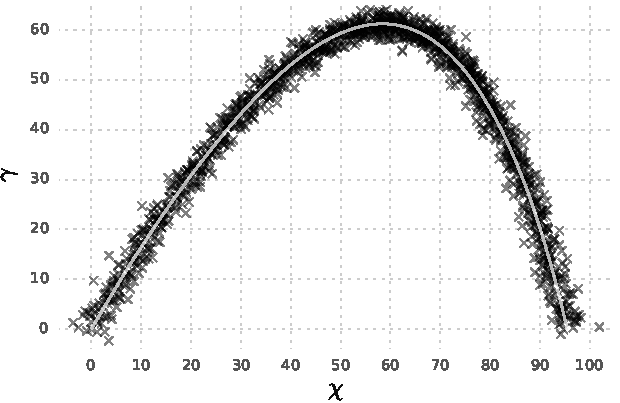
\includegraphics{img/ballistic_trajectory}%
	\caption{%
	A simulation of the trajectory
	of the projectile in model~\eqref{eq:ballistic_model}.
   	The measurements are denoted with crosses. %
   	}
	\label{fig:ballistic2D_simulation}
 \end{figure}

The linear-Gaussian SSM can now be written as
\begin{align}
	\begin{aligned}
	\x_k &= \v{A}\xkk+\v{u}+\v{L}\v{v}_{k-1}, & \v{v}_{k-1} &\sim \N{\v{0}}{\bm{\sigma_1^{2} & \\ & \sigma_2^{2}}}\\
	\yk &= \v{H}\xk+\v{r}_k, & 					\v{r}_k 	&\sim \N{\v{0}}{\sigma_r^2\v{I}},
	\end{aligned}\label{eq:ballistic_model}
\end{align}
where
\begin{align*}
	\v{A}&=\bm{
	1& \tau & 	& 		\\
	 &	1	& 	&		\\
	 &		& 1	& \tau 	\\
	 &		&	& 1
	}\\
	\v{u} &= \bm{ & g_1 &  & g_2}^\tr\\
	\v{L} &= \bm{\tau & 1 & &\\ & & \tau & 1}^\tr\\
	\v{H} &= \bm{1 & & &\\ & & 1 &}
\end{align*}
If we wish to replace $\v{L}v_{k-1}$ with the more familiar $\v{q}_{k-1}$,
then $\v{q}_{k-1}\sim \N{\v{0}}{\v{Q}}$ where
\begin{align}
	\v{Q} &= \v{L}\bm{\sigma_1^{2} & \\ & \sigma_2^{2}}\v{L}^\tr 
	%\sigma_1^2\bm{\frac{\tau^4}{4} & \frac{\tau^3}{2} &
	%\frac{\tau^2}{2}\\
	%\frac{\tau^3}{2} & \tau^2 & \tau\\ \frac{\tau^2}{2} & \tau & 1}
	\label{eq:ballistic_Q}
\end{align}
Additionally, the initial state $\x_0$ is assumed to be normally
distributed with $\N{\gv\mu_0}{\v{I}}$, where
\begin{align}
	\gv\mu_0 &= \bm{0 & \cos(\alpha_0)v_0 & 0 & \sin(\alpha_0)v_0}^\tr\\
	%\gv\Sigma_0 &= \mathrm{diag}\big(\bm{0 & 10^2 & 0 & 0 & 10^2 & 0}\big).
	\label{eq:ballistic_prior}
\end{align}
In other words, we assume the covariance matrix fully known
and specify further that the initial position and velocity
are deterministic and known.

Next we will focus on simulating measurements from the model and then estimating
the model parameters. The parameters of the initial distribution are chosen as
$\alpha_0 = \ang{50}$ and $v_0 = \SI{40}{m/s}$ and the initial state $\x_0$ is then
drawn from $\N{\gv\mu_0}{\gv\Sigma_0}$. The amount of drift in the gravitational force 
is controlled by the parameters $\sigma_1$ and $\sigma_2$.
These determine the standard deviations in the horizontal and vertical
components of the force per a single time step of duration $\tau$.
We will set 
\begin{align}
	\sigma_1&=\tau\,\si{m/s^2}\\
	\sigma_2&=\SI{0}{m/s^2}.
\end{align} 
%
Figure~\ref{fig:ballistic2D_simulation} presents  a simulated dataset, 
which is drawn from the two dimensional ballistic model with the aforementioned parameter
values.



Let us then proceed to maximum likelihood static parameter estimation. The training
data will be the simulated data, so that the true parameter values are the ones presented
earlier. In this case the most interesting parameter is probably the initial velocity,
i.e the angle $\alpha_0\in(0,\sfrac{\pi}{2})$ and the magnitude $v_0$, since it determines
the trajectory to a high degree.

 
Let us collect the parameters in the set $\Th=\brac{\sigma_1,\sigma_2,\sigma_r}$.

\parencite{ristic2004beyond,Ratna2008,Lindsten2010}
 %
% To demonstrate filtering and smoothing, the filtering distributions were
% computed with the Kalman filter of section~\ref{sec:kalman_filter} and the smoothing distributions with
% the RTS smoother of section~\ref{sec:rts_smoother}. The results of the simulation are presented in
% Figure~\ref{fig:ballistic}. The uncertainty in the filtering distributions is noticeably larger
% when compared to the smoothing distributions, since the smoothing distributions
% include the information of the ``future'' measurements in addition to the past and the current ones.
% \todo{analyze the figure a bit more} 

% \begin{figure}[htb]%
%     \centering%
%     \begin{subfigure}[t]{0.5\textwidth}%
%     	\centering%
%     	\caption{EM}\label{fig:ballistic_lh_em}%
%     	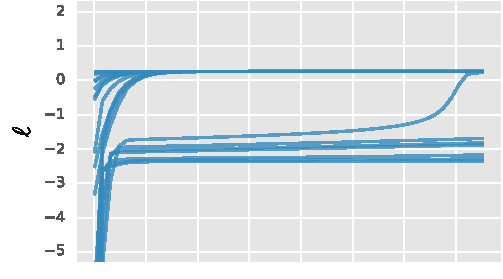
\includegraphics[width=\textwidth]{img/ballistic_lh_em}%
%     \end{subfigure}%
%     \begin{subfigure}[t]{0.5\textwidth}%
%     	\centering%
%     	\caption{BFGS}\label{fig:ballistic_lh_bf}%
% 		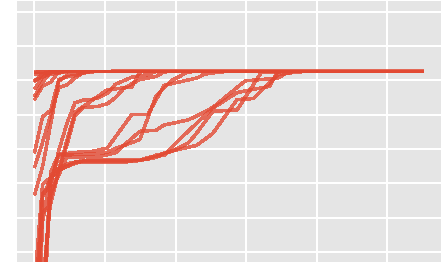
\includegraphics[width=\textwidth]{img/ballistic_lh_bf}%
%     \end{subfigure}%
% 	\caption{Convergence of the likelihood with EM and BFGS}
% 	\label{fig:ballistic_lh}
%  \end{figure}
 
 \begin{figure}[htb]%
    \centering%
    \makebox[\textwidth]{%
    \begin{subfigure}[t]{0.5\textwidth+0.4in}%
    	\caption{EM}
    	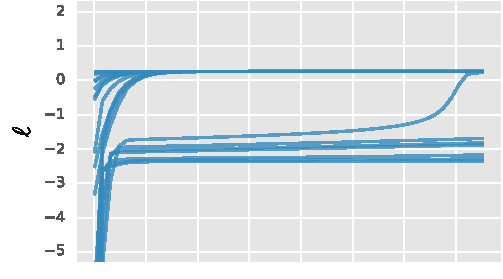
\includegraphics{img/ballistic_lh_em}%
    	%\caption{Convergence of the likelihood with EM}%
		%\label{fig:ballistic_lh_em}%
    \end{subfigure}%
    \begin{subfigure}[t]{0.5\textwidth+0.4in}%
		\caption{BFGS}
		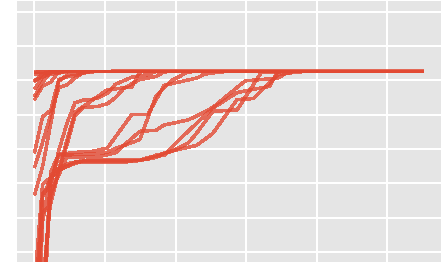
\includegraphics{img/ballistic_lh_bf}%
    	%\caption{Convergence of the likelihood with BFGS}%
		%\label{fig:ballistic_lh_bf}%
    \end{subfigure}}\\%
    \makebox[\textwidth]{%
    \begin{subfigure}[t]{0.5\textwidth+0.4in}%
    	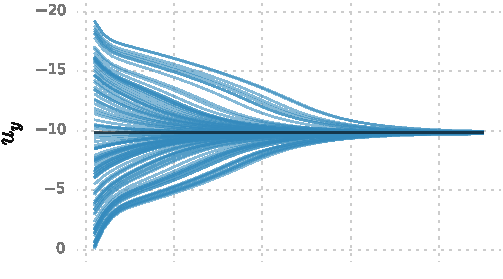
\includegraphics{img/ballistic_em_uy}%
    	%\caption{Convergence of the likelihood with EM}%
		%\label{fig:ballistic_lh_em}%
    \end{subfigure}%
    \begin{subfigure}[t]{0.5\textwidth+0.4in}%
		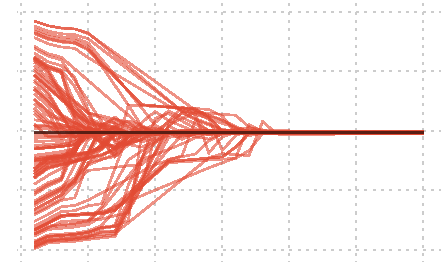
\includegraphics{img/ballistic_bf_uy}%
    	%\caption{Convergence of the likelihood with BFGS}%
		%\label{fig:ballistic_lh_bf}%
    \end{subfigure}}\\%
    \makebox[\textwidth]{%
    \begin{subfigure}[t]{0.5\textwidth+0.4in}%
    	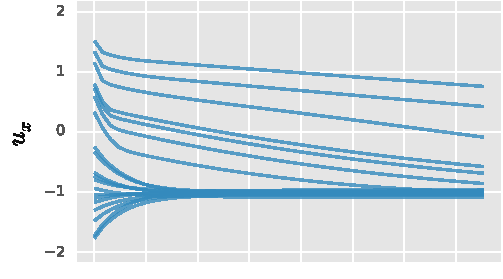
\includegraphics{img/ballistic_em_ux}%
    	%\caption{Convergence of the likelihood with EM}%
		%\label{fig:ballistic_lh_em}%
    \end{subfigure}%
    \begin{subfigure}[t]{0.5\textwidth+0.4in}%
		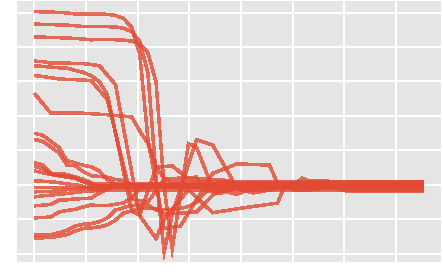
\includegraphics{img/ballistic_bf_ux}%
    	%\caption{Convergence of the likelihood with BFGS}%
		%\label{fig:ballistic_lh_bf}%
    \end{subfigure}}\\%
    \makebox[\textwidth]{%
	\begin{subfigure}[b]{0.5\textwidth+0.4in}%
    	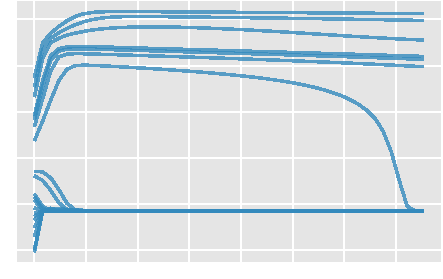
\includegraphics{img/ballistic_em_r}%
    	%\caption{Convergence of the likelihood with EM}%
		%\label{fig:ballistic_lh_em}%
    \end{subfigure}%
    \begin{subfigure}[b]{0.5\textwidth+0.4in}%
		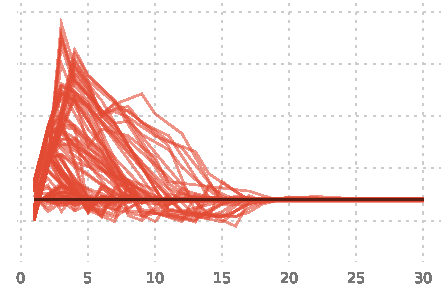
\includegraphics{img/ballistic_bf_r}%
    	%\caption{Convergence of the likelihood with BFGS}%
		%\label{fig:ballistic_lh_bf}%
    \end{subfigure}}%
    \caption{Convergence of the likelihood with EM and BFGS}\label{fig:ballistic_est}
 \end{figure}
 

\clearpage


%%%%%%%%%%%%%%%%%%%%%%%%%%%%%%%%%%%%%%%%%%%%%%%%%%%%%%%%%%%%%%%%
%%%%%%%%%%%%%%%%%%%% HEART %%%%%%%%%%%%%%%%%%%%%%%%%%%%%%%%%%%%%
%%%%%%%%%%%%%%%%%%%%%%%%%%%%%%%%%%%%%%%%%%%%%%%%%%%%%%%%%%%%%%%%

\subsection{Electrocardiograph analysis}

The second demonstration is concerned with a nonlinear model for
electrocardiograph (ECG) data, a short sequence of which is presented
in Figure~\ref{fig:ecg_data}. A realistic model for this data 
should take into account the quasi-periodic nature of ECG data,
i.e. the frequency must be allowed to vary with time.
Following the ideas in \textcite{Sarkka2012}, one possibility
is to write the model as a superposition of noisy resonators
with time-varying frequencies.

In continous time we can write a stochastic differential equation
for the $n$:th harmonic as
\begin{align}
	 \ddot{c}_n(t)&= -\omega(t)^2c_n(t)+\varepsilon_n(t),
	 %\dod[2]{c_n(t)}{t}
	\label{eq:noisy_resonator}
\end{align}
where $c_n(t)$ is the displacement from equilibrium at time $t$.
The angular velocity $\omega$ is related to the frequency $f$
by $\omega(t)=2\pi f(t)$ and  $\varepsilon_n(t)$ is additive
white noise with spectral density $q_n$. For constant frequency and
zero spectral density, the solution of Equation~\eqref{eq:noisy_resonator}
is well known to be $c_n(t)=\exp(i n \omega t+\phi_n)$, where $\phi_n\in\field{C}$ depends on 
the initial conditions.

Writing Equation~\eqref{eq:noisy_resonator} as a vector valued first order differential equation
and dividing the noise and the signal derivative by $n\omega(t)$, we get
\begin{align}
	\dod{}{t}\bm{c_n(t) \\ \widehat{\dot{c}}_n(t)} &= \bm{0 & \omega(t)^2 \\ -\omega(t) 0}\bm{c_n(t) \\
	\widehat{\dot{c}}_n(t)}+\bm{0\\1}
	\widehat{\varepsilon}_n(t).
	\label{eq:noisy_resonator_vec}
\end{align}
As explained in \textcite{Sarkka2012}, even if Equation~\eqref{eq:noisy_resonator_vec} is not an exact
representation of Equation~\eqref{eq:noisy_resonator}, its discretized version has more appealing
properties than that of the exact version. Furthermore, the process noise can account for some
modeling errors. 

Discretizing Equation~\eqref{eq:noisy_resonator_vec} at equispaced points $\brac{t_k}_{k=1}^T$
with interval $\tau$ and assuming $\omega(t)=\omega(t_k)\equiv \omega_k$ when $t\in\brak{t_k,t_{k+1}}$,
we get the following dynamic model for displacement $x^{(n)}$:
\begin{align}
	\bm{x_k^{(n)} \\ \dot{x}_k^{(n)}} &\sim 
	\N{\bm{\cos(n\omega_k) & \sin(n\omega_k) \\% 
	   -\sin(n\omega_k) & \cos(n\omega_k)}
	   \bm{x_{k-1}^{(n)} \\ \dot{x}_{k-1}^{(n)}}}
	  {\bm{0 & 0 \\ 0 & \tau q_x}}.
	\label{eq:dynamic_displacement}
\end{align}
We assume that $\omega_k$ is part of the state and assume its dynamics obey the previously introduced first order
random walk model (with $a=1$):
\begin{align}
	\omega_k \sim \N{\omega_{k-1}}{\tau q_\omega}.
	\label{eq:omega_ar}
\end{align}
The joint dynamic model of $m$ harmonics and $\omega_k$ is then
\begin{align}
	\underbrace{\bm{\omega_k \\ x_k^{(1)} \\ \dot{x}_k^{(1)} \\ \vdots \\  x_k^{(m)} \\ \dot{x}_k^{(m)} }}_{\xk} 
	=
	%\N{
	\underbrace{\bm{1&&&&&\\
		& \cos(\omega_k) & \sin(\omega_k) &&&\\% 
	    &-\sin(\omega_k) & \cos(\omega_k) &&&\\
	    &				  &					& \ddots & &\\
	 &&&& \cos(m\omega_k) & \sin(m\omega_k) \\% 
	 &&&&-\sin(m\omega_k) & \cos(m\omega_k) \\
	}
	\bm{\omega_k \\ x_{k-1}^{(1)} \\ \dot{x}_{k-1}^{(1)} \\ \vdots \\  x_{k-1}^{(m)} \\ \dot{x}_{k-1}^{(m)} }}_{\ffi}
	%}{
	%\v{Q}
	%},
	+ \v{q}_{k-1}
	\label{eq:harmonic_joint}
\end{align}
where
\begin{align}
	\q_{k-1}\sim\N{\v{0}}{\tau\bm{q_\omega&&&&&\\ & 0 &&&& \\ && q_x &&& \\ &&& \ddots && \\ &&&& 0 & \\ &&&&& q_x}}
	\label{tablelabel}
\end{align}


 
 \begin{figure}[htb]%
    \centering%
    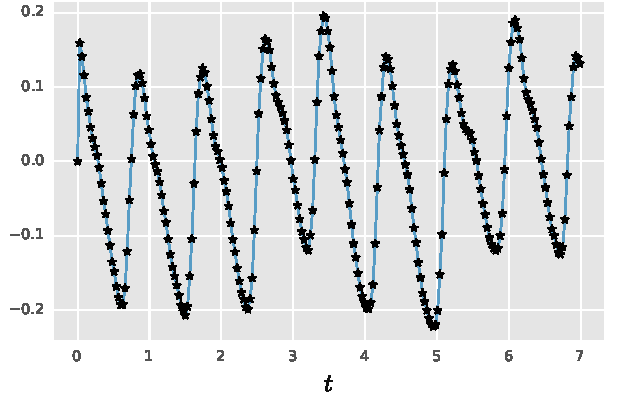
\includegraphics{img/harmonic_trajectory}%
	\caption{%
	A short sequence of the ECG data. %
   	}
	\label{fig:ecg_data}
 \end{figure}
 
 \begin{figure}[htb]%
    \centering%
    \makebox[\textwidth]{%
    \begin{subfigure}[t]{0.5\textwidth+0.4in}%
    	\caption{EM}
    	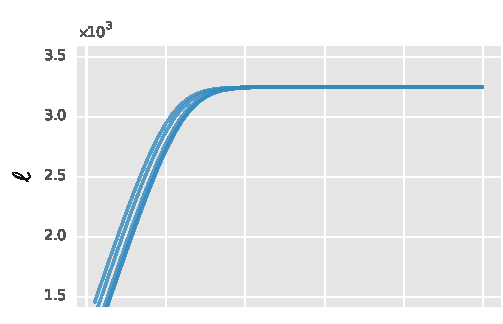
\includegraphics{img/harmonic_em_lh}%
    	%\caption{Convergence of the likelihood with EM}%
		%\label{fig:harmonic_lh_em}%
    \end{subfigure}%
    \begin{subfigure}[t]{0.5\textwidth+0.4in}%
		\caption{BFGS}
		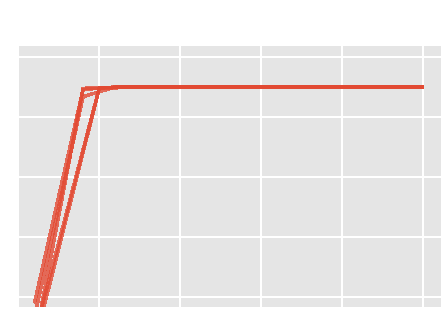
\includegraphics{img/harmonic_bf_lh}%
    	%\caption{Convergence of the likelihood with BFGS}%
		%\label{fig:harmonic_lh_bf}%
    \end{subfigure}}\\%
    \makebox[\textwidth]{%
    \begin{subfigure}[t]{0.5\textwidth+0.4in}%
    	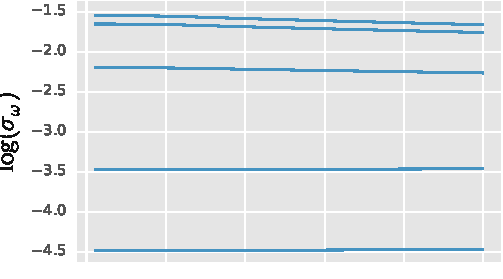
\includegraphics{img/harmonic_em_lqw}%
    	%\caption{Convergence of the likelihood with EM}%
		%\label{fig:harmonic_lh_em}%
    \end{subfigure}%
    \begin{subfigure}[t]{0.5\textwidth+0.4in}%
		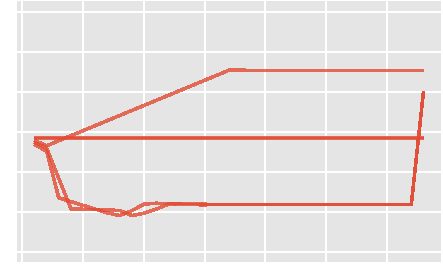
\includegraphics{img/harmonic_bf_lqw}%
    	%\caption{Convergence of the likelihood with BFGS}%
		%\label{fig:harmonic_lh_bf}%
    \end{subfigure}}\\%
    \makebox[\textwidth]{%
    \begin{subfigure}[t]{0.5\textwidth+0.4in}%
    	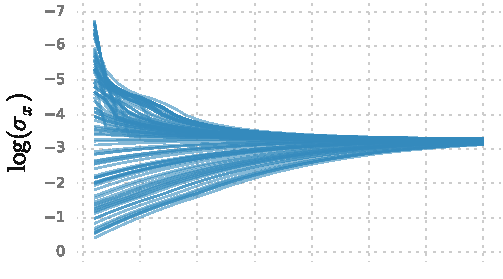
\includegraphics{img/harmonic_em_lqx}%
    	%\caption{Convergence of the likelihood with EM}%
		%\label{fig:harmonic_lh_em}%
    \end{subfigure}%
    \begin{subfigure}[t]{0.5\textwidth+0.4in}%
		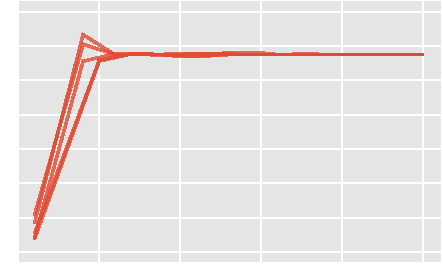
\includegraphics{img/harmonic_bf_lqx}%
    	%\caption{Convergence of the likelihood with BFGS}%
		%\label{fig:harmonic_lh_bf}%
    \end{subfigure}}%\\%
%     \makebox[\textwidth]{%
% 	\begin{subfigure}[b]{0.5\textwidth+0.4in}%
%     	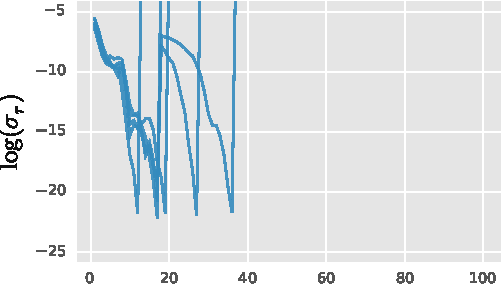
\includegraphics{img/harmonic_em_lr}%
%     	%\caption{Convergence of the likelihood with EM}%
% 		%\label{fig:harmonic_lh_em}%
%     \end{subfigure}%
%     \begin{subfigure}[b]{0.5\textwidth+0.4in}%
% 		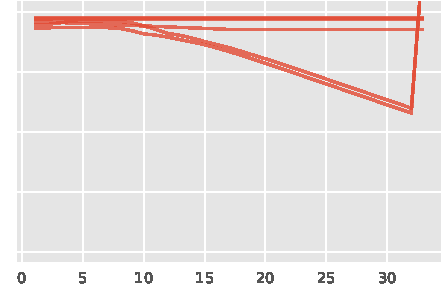
\includegraphics{img/harmonic_bf_lr}%
%     	%\caption{Convergence of the likelihood with BFGS}%
% 		%\label{fig:harmonic_lh_bf}%
%     \end{subfigure}}%
    \caption{Convergence of the likelihood and estimates with EM and BFGS}\label{fig:harmonic_est}
 \end{figure}

\section{Conclusion}
\todo{shortcomings of Gaussian filtering}
\todo{Dual and joint filtering}
\todo{particle filtering}
\parencite{Haykin2001}
\parencite{Kantas2009,doucet2001sequential,Gordon1993,Lindsten2010}


	
\clearpage
\listoftodos
\clearpage
\appendix
\numberwithin{equation}{section}
\numberwithin{lemma}{section}
\section{Additional material}
\subsection{Properties of the Gaussian distribution}
\begin{lemma} \label{lemma:gaussian_joint}
Suppose $\x\in\R^n$ and $\y\in\R^m$ have the distributions
\begin{align*}
	\Pdf{\x}&= \N[\x]{\v{m}}{\v{P}} \\
	\Pdf{\y}{\x}&= \N[\y]{\v{H}\x+\v{u}}{\v{R}}.
\end{align*}
Then the joint distribution is
\begin{align*}
	\Pdf{\begin{bmatrix}
		\x\\
		\y
	\end{bmatrix}}&=
	\N[\bm{\x\\\y}]{
	\begin{bmatrix}
		\v{m}\\
		\v{H}\v{m}+\v{u}
	\end{bmatrix}
	}{
	\begin{bmatrix}
		\v{P}&\v{P}\v{H}^\tr\\
		\v{H}\v{P}&\v{H}\v{P}\v{H}^\tr+\v{R}\\
	\end{bmatrix}
	}
\end{align*}
\end{lemma}
\begin{proof}
\begin{align}
	\E{\y}&=\defint{}{}{\y\,\Pdf{\y}}{\y} \nonumber\\
	&=\defint{}{}{\y\Big(\!\defint{}{}{\Pdf{\y}{\x}\Pdf{\x}}{\x}\Big)}{\y}\nonumber\\
	&\mbox{{\small (change the order of integration according to Fubini's theorem)}}\nonumber\\
	&=\E{\E{\y\mid\x}}\\
	%&=\defint{}{}{\fparen*{\v{H}\x+\v{u}}\Pdf{\x}}{\x}\label{eq:mean_int},\\
	&=\v{H}\v{m}+\v{u}\\
%\end{align}
%\begin{align}
	\var{\y}&=\defint{}{}{\fparen*{\y-\E{\y}}\fparen*{\y-\E{\y}}^\tr\Pdf{\y}{\x}\Pdf{\x}}{\y}{\x} \nonumber\\
	%&=\defint{}{}{\fparen*{\y-\E{\y}}\fparen*{\y-\E{\y}}^\tr\defint{}{}{\Pdf{\y}{\x}\Pdf{\x}}{\y}}{\x} \nonumber\\
	&=\E{\E{\y\mid\x}\E{\y\mid\x}^\tr}-\E{\E{\y\mid\x}}\E{\E{\y\mid\x}}^\tr \nonumber \\
&\quad+\defint{}{}{\fparen*{\y-\E{\y\mid\x}}\fparen*{\y-\E{\y\mid\x}}^\tr\Pdf{\y}{\x}\Pdf{\x}}{\y}{\x} \nonumber \\
	&= \var{\E{\y\mid\x}}+\E{\var{\y\mid\x}}\\
	&= \v{H}\v{P}\v{H}^\tr+\v{R}\\
%\end{align}
%\begin{align}
	\cov{\x}{\y}&=\defint{}{}{\fparen[\big]{\x-\E{\x}}\fparen[\big]{\y-\E{\y}}^\tr\Pdf{\x}\Pdf{\y}{\x}}{\x}{\y} \nonumber\\
	&=\defint{}{}{\fparen[\big]{\x-\E{\x}}\fparen[\big]{\E{\y\mid\x}-\E{\y}}^\tr\Pdf{\x}}{\x} \nonumber\\
	&=\defint{}{}{\fparen[\big]{\x-\v{m}}\fparen[\big]{\x-\v{m}}^\tr\v{H}^\tr\Pdf{\x}}{\x} \nonumber\\
	&=\v{P}\v{H}^\tr
\end{align}%

\end{proof}
\begin{lemma} \label{lemma:gaussian_cond}
Suppose $\x\in\R^n$ and $\y\in\R^m$ have the joint distribution
\begin{align*}
	\Pdf{\begin{bmatrix}
		\x\\
		\y
	\end{bmatrix}}&=
	\N[\bm{\x\\\y}]{
	\begin{bmatrix}
		\v{a}\\
		\v{b}
	\end{bmatrix}
	}{
	\begin{bmatrix}
		\v{A}&\v{C}\\
		\v{C}^\tr&\v{B}
	\end{bmatrix}
	}.
\end{align*}
Then the marginal and conditional distributions are given by
\begin{align*}
	\Pdf{\x} &= \N[\x]{\v{a}}{\v{A}}\\
	\Pdf{\y} &= \N[\x]{\v{b}}{\v{B}}\\
	\Pdf{\x}{\y}&= \N[\x][\displaystyle]{\v{a}+\v{C}\v{B}^{-1}\fparen*{\v{y}-\v{b}}}{\v{A}-\v{C}\v{B}^{-1}\v{C}^\tr}\\
	\Pdf{\y}{\x}&= \N[\x][\displaystyle]{\v{b}+\v{C}^\tr\v{A}^{-1}\fparen*{\v{x}-\v{a}}}{\v{B}-\v{C}^\tr\v{A}^{-1}\v{C}}
\end{align*}
\end{lemma}

\clearpage
\printbibliography
\end{document}

